% Options for packages loaded elsewhere
\PassOptionsToPackage{unicode}{hyperref}
\PassOptionsToPackage{hyphens}{url}
\PassOptionsToPackage{dvipsnames,svgnames,x11names}{xcolor}
%
\documentclass[
  letterpaper,
  DIV=11,
  numbers=noendperiod,
  oneside]{scrartcl}

\usepackage{amsmath,amssymb}
\usepackage{iftex}
\ifPDFTeX
  \usepackage[T1]{fontenc}
  \usepackage[utf8]{inputenc}
  \usepackage{textcomp} % provide euro and other symbols
\else % if luatex or xetex
  \usepackage{unicode-math}
  \defaultfontfeatures{Scale=MatchLowercase}
  \defaultfontfeatures[\rmfamily]{Ligatures=TeX,Scale=1}
\fi
\usepackage{lmodern}
\ifPDFTeX\else  
    % xetex/luatex font selection
\fi
% Use upquote if available, for straight quotes in verbatim environments
\IfFileExists{upquote.sty}{\usepackage{upquote}}{}
\IfFileExists{microtype.sty}{% use microtype if available
  \usepackage[]{microtype}
  \UseMicrotypeSet[protrusion]{basicmath} % disable protrusion for tt fonts
}{}
\makeatletter
\@ifundefined{KOMAClassName}{% if non-KOMA class
  \IfFileExists{parskip.sty}{%
    \usepackage{parskip}
  }{% else
    \setlength{\parindent}{0pt}
    \setlength{\parskip}{6pt plus 2pt minus 1pt}}
}{% if KOMA class
  \KOMAoptions{parskip=half}}
\makeatother
\usepackage{xcolor}
\usepackage[left=1in,marginparwidth=2.0666666666667in,textwidth=4.1333333333333in,marginparsep=0.3in]{geometry}
\setlength{\emergencystretch}{3em} % prevent overfull lines
\setcounter{secnumdepth}{-\maxdimen} % remove section numbering
% Make \paragraph and \subparagraph free-standing
\makeatletter
\ifx\paragraph\undefined\else
  \let\oldparagraph\paragraph
  \renewcommand{\paragraph}{
    \@ifstar
      \xxxParagraphStar
      \xxxParagraphNoStar
  }
  \newcommand{\xxxParagraphStar}[1]{\oldparagraph*{#1}\mbox{}}
  \newcommand{\xxxParagraphNoStar}[1]{\oldparagraph{#1}\mbox{}}
\fi
\ifx\subparagraph\undefined\else
  \let\oldsubparagraph\subparagraph
  \renewcommand{\subparagraph}{
    \@ifstar
      \xxxSubParagraphStar
      \xxxSubParagraphNoStar
  }
  \newcommand{\xxxSubParagraphStar}[1]{\oldsubparagraph*{#1}\mbox{}}
  \newcommand{\xxxSubParagraphNoStar}[1]{\oldsubparagraph{#1}\mbox{}}
\fi
\makeatother


\providecommand{\tightlist}{%
  \setlength{\itemsep}{0pt}\setlength{\parskip}{0pt}}\usepackage{longtable,booktabs,array}
\usepackage{calc} % for calculating minipage widths
% Correct order of tables after \paragraph or \subparagraph
\usepackage{etoolbox}
\makeatletter
\patchcmd\longtable{\par}{\if@noskipsec\mbox{}\fi\par}{}{}
\makeatother
% Allow footnotes in longtable head/foot
\IfFileExists{footnotehyper.sty}{\usepackage{footnotehyper}}{\usepackage{footnote}}
\makesavenoteenv{longtable}
\usepackage{graphicx}
\makeatletter
\def\maxwidth{\ifdim\Gin@nat@width>\linewidth\linewidth\else\Gin@nat@width\fi}
\def\maxheight{\ifdim\Gin@nat@height>\textheight\textheight\else\Gin@nat@height\fi}
\makeatother
% Scale images if necessary, so that they will not overflow the page
% margins by default, and it is still possible to overwrite the defaults
% using explicit options in \includegraphics[width, height, ...]{}
\setkeys{Gin}{width=\maxwidth,height=\maxheight,keepaspectratio}
% Set default figure placement to htbp
\makeatletter
\def\fps@figure{htbp}
\makeatother
% definitions for citeproc citations
\NewDocumentCommand\citeproctext{}{}
\NewDocumentCommand\citeproc{mm}{%
  \begingroup\def\citeproctext{#2}\cite{#1}\endgroup}
\makeatletter
 % allow citations to break across lines
 \let\@cite@ofmt\@firstofone
 % avoid brackets around text for \cite:
 \def\@biblabel#1{}
 \def\@cite#1#2{{#1\if@tempswa , #2\fi}}
\makeatother
\newlength{\cslhangindent}
\setlength{\cslhangindent}{1.5em}
\newlength{\csllabelwidth}
\setlength{\csllabelwidth}{3em}
\newenvironment{CSLReferences}[2] % #1 hanging-indent, #2 entry-spacing
 {\begin{list}{}{%
  \setlength{\itemindent}{0pt}
  \setlength{\leftmargin}{0pt}
  \setlength{\parsep}{0pt}
  % turn on hanging indent if param 1 is 1
  \ifodd #1
   \setlength{\leftmargin}{\cslhangindent}
   \setlength{\itemindent}{-1\cslhangindent}
  \fi
  % set entry spacing
  \setlength{\itemsep}{#2\baselineskip}}}
 {\end{list}}
\usepackage{calc}
\newcommand{\CSLBlock}[1]{\hfill\break\parbox[t]{\linewidth}{\strut\ignorespaces#1\strut}}
\newcommand{\CSLLeftMargin}[1]{\parbox[t]{\csllabelwidth}{\strut#1\strut}}
\newcommand{\CSLRightInline}[1]{\parbox[t]{\linewidth - \csllabelwidth}{\strut#1\strut}}
\newcommand{\CSLIndent}[1]{\hspace{\cslhangindent}#1}

\KOMAoption{captions}{tableheading}
\makeatletter
\@ifpackageloaded{caption}{}{\usepackage{caption}}
\AtBeginDocument{%
\ifdefined\contentsname
  \renewcommand*\contentsname{Table of contents}
\else
  \newcommand\contentsname{Table of contents}
\fi
\ifdefined\listfigurename
  \renewcommand*\listfigurename{List of Figures}
\else
  \newcommand\listfigurename{List of Figures}
\fi
\ifdefined\listtablename
  \renewcommand*\listtablename{List of Tables}
\else
  \newcommand\listtablename{List of Tables}
\fi
\ifdefined\figurename
  \renewcommand*\figurename{Figure}
\else
  \newcommand\figurename{Figure}
\fi
\ifdefined\tablename
  \renewcommand*\tablename{Table}
\else
  \newcommand\tablename{Table}
\fi
}
\@ifpackageloaded{float}{}{\usepackage{float}}
\floatstyle{ruled}
\@ifundefined{c@chapter}{\newfloat{codelisting}{h}{lop}}{\newfloat{codelisting}{h}{lop}[chapter]}
\floatname{codelisting}{Listing}
\newcommand*\listoflistings{\listof{codelisting}{List of Listings}}
\makeatother
\makeatletter
\makeatother
\makeatletter
\@ifpackageloaded{caption}{}{\usepackage{caption}}
\@ifpackageloaded{subcaption}{}{\usepackage{subcaption}}
\makeatother
\makeatletter
\@ifpackageloaded{sidenotes}{}{\usepackage{sidenotes}}
\@ifpackageloaded{marginnote}{}{\usepackage{marginnote}}
\makeatother

\ifLuaTeX
\usepackage[bidi=basic]{babel}
\else
\usepackage[bidi=default]{babel}
\fi
\babelprovide[main,import]{english}
% get rid of language-specific shorthands (see #6817):
\let\LanguageShortHands\languageshorthands
\def\languageshorthands#1{}
\ifLuaTeX
  \usepackage{selnolig}  % disable illegal ligatures
\fi
\usepackage{bookmark}

\IfFileExists{xurl.sty}{\usepackage{xurl}}{} % add URL line breaks if available
\urlstyle{same} % disable monospaced font for URLs
\hypersetup{
  pdftitle={If I Only Had A Brain: Memory Retention After Decapitation and Regeneration in Planaria},
  pdfauthor={Francis Forde},
  pdflang={en},
  pdfkeywords={Memory, Learning, Planaria, Reinstatement, Cocaine, Behaviour},
  colorlinks=true,
  linkcolor={blue},
  filecolor={Maroon},
  citecolor={Blue},
  urlcolor={Blue},
  pdfcreator={LaTeX via pandoc}}


\title{If I Only Had A Brain: Memory Retention After Decapitation and
Regeneration in Planaria}
\author{Francis Forde}
\date{}

\begin{document}
\maketitle
\begin{abstract}
XX
\end{abstract}


\section{Introduction}\label{introduction}

\begin{itemize}
\item
  Brief intrduction to area
\item
  Knowldge gap
\item
  How I addressed this
\item
  What I found
\item
  What this might mean
\end{itemize}

\section{Background}\label{background}

A brain in isolation is just a clump of extravagant cells. A brain earns
its keep through interacting with the body and the external world. It is
among these brain-environment interactions that an organism can set and
acheive goals and, ulitimately, carve a pathway to survival. But brains
operate in the dark. Their only insight into the on-goings of the world
is through delicately placed sensory organs such as eyes, nose and ears.
The sensory technology that each organisms possess', what pilosophers
call its sensorium, differs across species. Some build a picture of the
world by capturing light using light sensitive proteins. Others live
where no light can penetrate and so must form their worldview using
other sensory modalities like exholocation. Notwithstanding these
differences, neuroscience (in collaboration with biology) seeks to
understand the suite of abilities each organism possesses, the neuronal
and molecular mechanisms which underpin these, and the factors that
determine when and why an organism deploys the behaviours in its
arsenal. When we use non-human organisms during scinetific inquiry, we
often do so while hopeing the knowledge gleaned will teach us something
about our own brains and bodies.

We now have at hand a broad tool set for inspecting the brain across
different time spans and at different levels of analysis. From looking
at activity within a single dendritic spine over microseconds to looking
at connectivity between different brain structures over many seconds. We
can even track changes in the size and number of individual spines on a
single dendrite over time -- impressive given the width of a spine is
100 times smaller than the thickness of a human hair. At the network
level, we are able to identify groups of neurons (ensembles) involved in
encoding and storing memory, and can use precise tools to excite or
inhibit those networks to alter an animals behaviour.

Our current experimental competency arose from many small steps. Before
we had the means to manipulate neurons and undestand their role in
memory, we had to make do with simple procedures like learning lists of
nonsense syllables or simple motor tasks. This research often utilised
patients who had conditions like amnesia or who had suffered some kind
of brain injury.This early research helped answer the question whether
memory is a unitary system or a suite of seperate systems which can be
dissociated. Distinctions such as episodic and procedural, as well as
short- and long-term emerged. Theoretical progress provided the
foundation upon which specialsied tools and procedures could be
developed to manipulate and characterise the biology of memory in its
different forms.

\subsection{Overview of key concepts in the field of learning and
memory}\label{overview-of-key-concepts-in-the-field-of-learning-and-memory}

\subsubsection{The meaning of memory and the different forms it
takes}\label{the-meaning-of-memory-and-the-different-forms-it-takes}

Generally speaking, memory is the embodiment of past experience which
shapes our future behaviour. Learning is the process of memory
acquisition. Though, it must be said that there may be as many different
definitions of learning and memory as there are papers published on the
topic. Barron et al. (\citeproc{ref-barron_embracing_2015}{2015})
surveyed the various uses of the term ``learning'' across disciplines
such as cognitive psychology, behavioural ecology, and machine learning
and identified at least 50 definitions (albeit with a lot of overlap).
Memory has been parceled into several distinct categories based on the
content of the information being stored. The major distinction is
between explicit (or declarative) and implicit (or procedural) memory
(\citeproc{ref-squire_memory_1987}{Squire 1987};
\citeproc{ref-schacter_memory_1994}{Schacter and Tulving 1994}) as shown
in Figure 1 below. Explicit memories are those accessible to
consciousness. Implicit memories refer to information that you cannot
consciously access. Explicit memory has been further subdivided into
episodic and semantic memory (Tulving, 1972). With episodic referring to
the rich experiential quality of personal memories, while semantic
relates to things that you know, but that lack an experiential component
(e.g.~facts about the world).

Memories can also be categorised on the temporal dimension. Atkinson and
Shiffrin (1968) proposed three memory stores: a sensory register, a
short term, and a long term store. This division is still usefully
applied in the field of learning and memory (e.g,
\citeproc{ref-miller_timescales_2024}{Miller and Constantinidis 2024}).
A temporal framing of memory reflects the learning process itself.
Learning is normally broken up into several stages, each building on
those before to further engrain the memory and expand its longevity (see
Section~\ref{sec-mechanisms} below) . Initially, information enters a
short term state and may alter behaviour and decision making in the
immediate future. However, most of the information that our brains
initially perceive -- all the light hitting our eyes, and all the
vibrations in the air registered by our ears -- is not retained. To
successfully retain this information it must be actively incorporated
into our biology and maintained so that it can be accessed or recalled
in perpetuity. To put it another way, the Information that is taken on
board but must undergo specific processes (known as consolidation) to
stave off the forgetting process.

These distinctions make a lot of sense when talking about memory in
humans. But it may not be immediately clear what relevance these
distinctions have when looking at other organisms. Most people do not
attribute rich episodic (experiential) memories to rodents, let alone
invertebrates. Yet, it is clear that even very simple organisms have the
capacity to learn and store varied types of memory; Ranging from basic
changes in a reflexes (habituation and sensitisation) to more complex
operant behaviours. Such distinctions may be particlalry relevent for
the phenomena of memory storage outside of the brain, as is the topic
pursued in this project. if, as the literature suggests, some memories
are able to be retained outside the brain (and perhaps outside the CNS)
these concepts may help us derive the bounds of which memory types hold
this property and which do not. It may be that procedural memories such
as non-associative responses are stored outside of neural networks. But
memories which are consciously accessible are only able to be stored
among complex ensembles of neurons in the brain. We do not yet know the
bounds of non-neuronal memory storage, if it truly exists. But armed
with these conceptual distinctions between types of memory, we can apply
tailored training techniques to find out what forms of learning persist
outside the brain and which do not.

\subsubsection{Associative and non-associative
learning}\label{associative-and-non-associative-learning}

Associative learning is learning the relationship between two stimuli.
One stimulus reliably precedes another, or a behaviour reliably precedes
a reward. Non-associative forms of learning captures learning about a
stimulus itself, but not in relation to other stimuli. This typically
takes the form of behavioural sensitization or habituation. If you were
to mildly shock my hand, I would withdraw it reflexively as it would be
startling. But with repeated administration of the shock over time, I
may come to learn that the shock is actually not that painful after all.
The size of my startle response decreased over time with repeated
exposure (habituation). I have learned something about the shock, but
have learned nothing about its relationship to other stimuli. To extend
this example to an associative form of learning, the shock could be
delivered after being shown a picture of a certain flower. I would
therefore associate (likely subconsciously) the flower imagery with a
negative experience, and would eventually display a fear startle to
presentations of the flower (tense up, squint my eyes, dip my head).
This captures the fact that I have learned a temporal association
between the flower and the shock. My body learns to prepare for the
before it arrives.

Classical conditioning and operant conditioning are two frequently used
forms of associative learning. Classical conditioning involves learning
an association between two or more stimuli, as in the flower/shock
example above. Operant conditioning differs from classical conditioning
in that rather than a stimulus (e.g.~shock) being paired with another
stimulus (flower), a behaviour comes to be associated with a desirable
outcome. For example, I learn that signing up to psychology experiments
often invovles being exposed to (mildly) irratting stimuli. This changes
the likelihood of that response being produced in the future. In other
words, I stop signing up as a participant. Good for me, not so good for
postgraduate students trying to complete their research.

\subsubsection{Maladaptive learning}\label{maladaptive-learning}

The examples outline above cover adpative learning. preparing for shocks
in the case of classical conditioning reduces the painfulness of the
stimuli. Avoiding experiments means that I am exposed to less
unnecessary irritants. These are of course simple toy examples, but real
life examples abound whereby our wellbeing and longevity is greatly
enhanced by learning from past experiences. A close call when crossing a
road (and the negative phsyiology experience that ensues) may increase
the likelihood of diligently looking both ways in the future before
crossing a road. These learning experiences allow us to persist in a
world full of novel and ancient dangers. But the capacity for learning
raises several vulnerabilities.

Learning has a darker side. Consider Rebecca's first experience with
heroine. Prior to consumption, Rebecca has heard about herione, but only
in the sense that she knows it is a harmful drug, that similar drugs are
used in a medical setting, and so on. She has no prior subjective
epxerince of its effects. But after several experiences with the drug at
parties, she learns about the intense sense of euphoria that comes from
taking the drug. Later on, Sarah starts to feel a strong motivation to
take the drug again, especially when she sees cues associated with the
drug (syringes, white powder). Without the capacity to form such
associations, addiction would not be an issue. Sarah would fail to
remember what actions led to such euphoric experiences, and no memories
would be recalled at the sight of drug paraphenalia. we can see that
addiction arises from the often useful ability to remember what past
actions and events resulted in positive and negative experiences. In
Rebecca's case, the euphoria that was experienced as positive in the
moment led to neurological rewiring, hijacking the cognitive system to
pursue herione in the face of adverse consequences in the future. This
is an unfortunate but common case of maladaptive learning.

Many aspects of poor mental health conditions, including aspects of
depression, PTSD, and anxiety, similarly rely on memory systems for
their development. Anxiety is especially relevant, as it involves the
worry or concern over some perceived threat. The threat has not yet
occurred, but to a person with anxiety, memory of past experience of
similar circumstances creates excessive fear and a sense of unease as
they imagine a similar negative outcome occurring in the future. By
understanding what leads to the creation of these associations between a
context and a negative outcome, memory research can then help us explore
ways to prevent anxiety-like responses in the future, and identify
methods to unlearn the initial negative association. But to understand

\subsubsection{Mechanisms of memory storage}\label{sec-mechanisms}

As described earlier, the process of acquiring a memory involves
transferring information from a short term store to a long term store.
The default process for all organisms is to forget information. In fact,
we probably forget most of the information we encounter. This is
evolutionarily sensible. Storing information takes energy, and attaining
energy comes at a price. Every organism therefore has a small number of
things about which it must dedicate a lot of attention towards to track
and understand. But most of the information it encounters, be it visual,
tactile, or olfactory, does not matter to it. A penguin cares about the
scent of a polar bear, but not about the small bug being crushed under
its foot. While a penguin's brain would process both to some degree, it
is not equally likely to remember both experiences and the contexts in
which they took place.

When discussing how information is stored, one becomes steeped in
complex biological pathways. Such pathways involve proteins interacting
with other proteins, proteins interacting with DNA, and the production
of new proteins. In the neurobiological literature, much of the
discussion around learning takes place at the level of synapses --
synapses being the points where two neurons interact. The axon from
neuron A attaches to a dendrite from neuron B and thus form a synapse.
Synapses are the locus of neuronal communication in the brain. At an
abstract level, learning is realised by information affecting neurons
such that they progress through a sequence of stages: acquisition,
stabalisation, consolidation and maintenance (see Rudy 2014 for a
digestible overview of each stage). There are complicated mechanisms
involved in each stage of learning, and not all the components are fully
understood. Despite that, the literature provides a good sense of many
important molecular events that are involved in the process of storing
information in the brain and being able to act on that information at a
later time point.

When some new bit of information has been processed by the brain, the
physical embodiment in the brain is often described as the ``memory
trace'' (Asok et al., 2019; Robins, 2023; Semon, 1921). An influx of
calcium (resulting from stimulation by an upstream neuron A) is
necessary for the initial \textbf{generation} of the memory trace. The
calcium interacts within the post-synaptic dendritic spine on neuron B
and leads to actin being broken down into smaller chunks. Actin helps
give structure to the spine. Breaking it down is a necessary step to
create room to fit more receptors into the post-synaptic membrane of
neuron B -- the membrane acts as the skin between the cell and the
watery world outside of the cell. Adding receptors to the membrane makes
the spine on neuron B more sensitive to the upstream firing of neuron A,
and thus more likely to itself fire an action potential in response. But
this rapid change in sensitivity (potentiation) is short lived. Without
additional actions, this potentiation will revert back to baseline.
\textbf{Stabalisation} of the trace requires expanding and strengthening
the actin network in the dendritic spine. The spine head is enlarged,
and the actin scaffolding is changes to make it less vulnerable to being
broken down (depolymerated). Furthermore, proteins in the cell membrane
called adhesion molecules help to couple the pre- and post-synaptic
neurons, improving the effectiveness of neurotransmission. These first
two stages, generation and stabalisation, establishthe memory in the
curreny of biologically material, but are not themselves enough to
ensure the memory stands the test of time. Much like a digital file that
you create and store on your local drive. It has been written and stored
in a meanignful way, but it can be easily lost if the hard drive is
damaged or the file is deleted by someone freeing up space for their own
documents. It is not until you back your files up to a network that you
can be confident in their future accessibility.

\textbf{Consolidation} is a unique step in the process of learning where
proteins enter the nucleus and establish a chain of events leading to
the productiong of new proteins. After entering the nucleus, the
proteins bind to DNA signal to the genome which leads to transcription
of new molecules (mRNA) that will then be turned into proteins, such as
receptors that can be inserted in the membrane. These instructions to
the genome to continually mint new proteins ensures a sufficient pool of
receptors and other elements are avaliable to keep the spine in a
potentiated (more sensitive) state. Finally, during the
\textbf{maintenance} stage this supply of membrane receptors is produced
and inserted into the membrane. and the typical dynamics of receptor
removal, where receptors are removed from the membrane and recycled, is
dampened. More excitatory receptors remain on the cell membrane which
ensures heightened sensitivity to signals from presynaptic neurons both
now and in the future.

\subsubsection{Memory research in animals and
invertebrates}\label{memory-research-in-animals-and-invertebrates}

Many organisms have found themselves being poked, prodded and leered at
as we attempted to understand the underlying mechanisms of memory. Scrub
jays, a bird sporting a bold blue coat and pointed black beak, have long
been subjects in studies investigating spatial memory because of their
food caching expertiese (Shettleworth \& Krebs, 1982). Rather
sophisticated methods have been used to study changes in hippocampal
volume with caching and the possibility of season-dependent changes in
hippocampal neurogenesis in caching birds (reviewed in Pravosudov,
2007). Rodents have also featured heavily in the experimental memory
literature (Ghafarimoghadam et al., 2022). Recent advances in
stimulation (e.g.~optogenetics; Goshen, 2014) and imaging
(e.g.~two-photon microscopy; Kawakam et al., 2015) have enabled us to
study representation of different types of memory at levels ranging from
individual synapses to neuronal ensembles.

Rodent models have been developed for tapping into spatial memory,
working memory, associative memory, recognition, and long term memory.
Most strikingly, the last two decades saw an intense exploration of
episodic memory in rodents. Episodic memory, at its essence, is the
ability to represent the past and draw on specific encoded events in a
manner akin to mental time travel (Tulving, 2002; Eacott \& Easton,
2007; Crystal, 2022). Intricate tasks have been developed which enable
rats to demonstrate memory for the context in which a stimulus had been
previously presented, and to disentangled this from mere familiarity
with the stimuli due to temporal proximity (Panoz-Brown et al., 2016).
However, the existence of episodic-like memory in non-human animals
remains debated ( Tulving (\citeproc{ref-tulving2005}{2005}); Hoerl and
McCormack (\citeproc{ref-hoerl2019}{2019}) ). The establishment of
procedures for identifying and manipulating complex episodic memory, by
optogenetic and other means, may help inform us on the type of
mechanisms (synaptic or molecular) likely to support episodic memory in
humans.

\begin{itemize}
\tightlist
\item
  Paragrapgh on primates in memory research?
\end{itemize}

These odd collection of experimental subjects supplied us with decades
of insights into learning processes and the nature of memory. But when
seeking to understand the precise molecular and structural changes that
underpin memory, the field first looked to invertebrates. The simplicity
of invertebrate neural architecture allowed researchers to account for
and track the entirety of the nervous system, and to observe functional
specificity of neurons. But simplicity is not the only benefit. By using
simpler organisms costs can be significantly reduced and environmental
variables can be more easily controlled. Moreover, ethical concerns are
relieved (albeit not completely removed) due to a lower porbability of
quantity and/or quality of sentience at this level.

While perhaps largely unknown outside of the sciences, Aplysia is a
celebrity among the invertebrates for its contribution to the
neurobiology of learning. Aplysia is a marine snail with a simple
nervous system. The abdominal ganglion (collection of neurons) of the
aplysia is home to the largest known neurons in nature (Moroz et
al.,2014). This makes it an ideal candidate for electrophysiology -- the
approach where neural activity is recorded by inserting electrodes into
cells or in the space surrounding cells. In aplysia. stimulation of the
siphon (used for transporting water in the body) leads to a defensive
retraction of the gill. Repeated stimulation leads to a decrease in the
intensity and length of the response, a simple form of non-associative
memory called habituation. This simple form of learning is not something
we typically care about . Yet, even this basic for of learning in
aplysia served as a useful platform for understanding the stages of
learning from acquisition through to consolidation described above,
which likely translate to and underpin more complex forms of memory that
we do care about in humans.

C. elegans is another organism which towers above most invertebrates in
its popularity. C. elegans gained prestige after it was the first
organisms to have its connectome mapped (White, Thomson \& Brenner,
1986). Understating the wiring of all 302 neurons in C. elegans provided
systems level insight into how an central nerveous system coordinates a
body to perform a suite of actions like movement, digestion, and
defensive behaviours. Though the scale of the nerveous system is small
compared to mammals, it revealed principles of neuronal organisation
which persist across brains of all sizes, principles such as reciprocal
inhibition to facilitate movement, computing at the level of the cell
for efficiency, and minimising the total length of neuronal wire
(Sterling \& Laughlin, 2015).

One of the most surprising findings from the study of learning and
behaviour in invertebrates is the complexity that can arise from a
paucity of neural cells. Consider that C. elegans has less connections
in its entire nervous system (\textasciitilde7000) than a single
mamillian pyramidal neuron has (Cook et al., 2019; Sterling \& Laughlin,
2016; Megı́as et al., 2001). Yet, this small neuronal setup is sufficient
to detect a variety of chemical and olfactory cues, navigate an
environment, escape threats and detect dynamic environmental signals
such as temperature and social crowding. Moreover, several thousand
connections can support a variety of learning including classical and
operant conditioning. And as we climb the ladder of neural complexity
from C. elegans to invertebrates like planaria, the cognitive
capabilities and potential insights multiply in suit.

\subsubsection{Planaria as a model
organism}\label{planaria-as-a-model-organism}

Planaria are a broad group of invertebrates which have become the
centerpiece for a number of scientific investigations. Planariar are
being used to investigate topics including regenerative biology (Karami
et al. (\citeproc{ref-karami2015}{2015})), toxicology (Li
(\citeproc{ref-li2008}{2008}); Hagstrom et al.
(\citeproc{ref-hagstrom2019}{2019}) ), radioprotective materials (
Ermakov et al. (\citeproc{ref-ermakov_planarians_2021}{2021})) addiction
(Raffa (\citeproc{ref-raffa2008}{2008})), and the effect of zero gravity
environments on morphology (Vista SSEP Mission 11 Team et al.
(\citeproc{ref-vistassepmission11team2018}{2018})). Planaria have built
niches across many ecological contexts and can be found across
salt-water, fresh-water and land environments. Land dwelling planaria
span up to half a meter long (Esser, 1981), whereas freshwater planaria,
which are more commonly used in behavioural research, are less than a
centimetre in length (Vásquez-Doorman, Escobedo \& Allende, 2022).

Planaria are bilaterians, they display bilateral symmetry across their
left and right sides (Sluys \& Riutort, 2018). Planaria exhibit
anterior-posterior polarity, such that their head can be distinguised
from the tail in both its structure and its behavioural repertoire.
While the tail end of a planarian rather uninteresting, the head
encompasses many useful features. Auricles, the sensory organs capable
of chemoreception, are what give the head of many planarian species its
triangular shape. These provide planaria with their ability to detect
food and noxious chemicals in the immediate environment. Eyespots, which
are the most discernible feature of planaria, sit atop the dorsal
surface of the head. These light-sensitive cell clusters enable planaria
to detect light intensity and its direction. Of particular interest to
neruoscientists, the planarian head encases a bilobed symmetrical brain
which coordinates activity throughout the body. This simple neural
structure is of special evolutionary significance as planaria are
thought to be the oldest organism to house an organised central nervous
system, or what we might label as a true brain (Pagán, 2014; Sarnat \&
Netsky 1985). In real terms, a planarian brain is drab compared to the
exuberance of the mammalian brain. But in relative terms, the
brain-to-body mass ratio of planarians is similar to that of a rat
(Best, 1983).

The planarian brain resembles an inverted U-shape (Agata et. al, 1998;
Sarnat \& Netsky, 1985) and has been estimated to contain between twenty
to thirty thousand neurons (Inoue, 2017, p.82). The brain exhibits nine
branches on each side which radiate out from the center. The lobes of
the brain form thin nerve cords at the posterior end. These chords
extend down the length of the body towards the tail, and together with
the brain, comprise the central nervous system. The left and right nerve
cords are connected by commissures which form a ladder-like structure
(Sluys \& Riutort, 2018). At first glance, the nerve chords do not have
the organisational compexity of the plaanrian brain. Judging purely from
apperances, the nerve chords should not be capable of performing complex
behaviour. However, It has been shown that even cells in the nerve
chords can take on the behavioural profile of a head, indicating that
the nerve chords are not simply axons innervating muscle (Le et al.,
2021).

Planarian neurons appear more similar in structure to those of
vertebrates than of other invertebrates. They feature spine-like
protrusions on dendrites (Sarnat \& Netsky, 1985; Petralia et al.,
2016). Just as in the CNS of vertebrates, multipolar neurons containing
many dendritic branches but a singular axon are common in the planarian.
Zooming in further, planarian neurons contain a variety of synaptic
vesicles, such as clear and dense-core variations, which resemble those
seen in vertebrate neurons (Oosaki \& Ishii, 1965). Most relevant to the
research described in this project, planaria produce many of the same
neurotransmitters and neuromodulators that we humans posses. These
include serotonin, dopamine, epinephrine, acetylcholine, GABA, glutamate
and opioid peptides (Sarnat \& Netsky, 1985; Welsh \& Williams, 1970;
Rawls et al., 2006; for a of planarian neurochemistry see Buttarelli et
al., 2008).

The physiologist August Krogh posited that ``You will find in the lower
animals mechanisms and adaptations of exquisite beauty and the most
surprising character'' (1929, p.203). The conservation of neurochemistry
in planaria is intriguing. But the primary feature which embodies
Krogh's dictum is the regenerative capability of planaria. Planaria
undergo a natural form of fission as part of their reproductive cycle.
They tear themselves in half, with each half then regrowing all the
necessary parts of its basic body plan to form a complete planarian
again. A form of reproductive immortality. Regeneration is not
completely novel in nature. Humans can regrow skin, and salamanders can
regrow amputated limbs. But what sets planaria apart from the rest of
the natural world is its ability to regrow its brain and central nervous
system. This regeneration is facilitated by adult pluripotent neoblast
cells which are found throughout the body (Neuhof et al., 2016). After
significant injury, these cells proliferate and undergo differentiation,
providing the cell types needed to restore organs, membranes, and neural
networks in the brain. This capability has drawn interest from medical
researchers for more than a century (Morgan, 1898; Child, 1941; Reddien,
2018), who realised that by understanding the factors that control
planarian regeneration, we may be able to artificially simulate these
processes in humans to restore limbs or neural structures after injury.
We have now reached the stage where business ventures like the company
Morphoceuticals are being established to apply lessons learnt from
planarian regeneration to rodents and, pending pre-clinical success,
eventually humans.

\subsubsection{Review of planarian memory
literature}\label{review-of-planarian-memory-literature}

In the early 1900's, a common belief was that invertebrates did not have
the cognitive means needed to learn. People conceded that perhaps local
tissue change may allow some acute form of memory. But this would
inevitably be erased or overwritten due to subsequent changes.
Invertebrates were thus thought to lack permanent memory systems. This
view is evident in the strong statement provide by Donald Jensen in the
1970s that ``no invertebrate, no matter how complex is capable of
showing `true learning'\,'' (quoted in Rilling p.~591). This view
established an artifical floor seperating the types of animals that are
suitable models of human cognition from those that are not. Because
invertebrates were off the table, researchers had to try and make
progress on the neurobiology of memory by starting with extremely
complicated animals like rodents. After many years in search of the
engram (the collection of neurons underlying a specific learning event),
this venture unearthed little if anything of value. A group of
psychologists including James McConnell in the 1970s were aware that
little progress was being made in this endevour. The group then moved
away from rodents and, looking past the anthropocentric restirctions
imposed on cognition, drifted towards invertebrates. Starting with much
simpler organisms would allow more insightful discoveries, as small
neural systems could be mapped and understood as a first step, while
complicated mammalian nervous systems could not. The situation was akin
to assembling a rocketship for exploring space before figuring out
commercial aviation within the earths atmosphere.

At first, McConnell and colleagues completed basic experiments showing
that planaria could learn to associate a light with a shock. Compared to
control subjects, trained planaria would exhibit more body contractions
in response to light (a conditioned stimulus) and also perform more
changes of direction. But criticism arose over the lack of controls in
these experiments. Later follow ups included blinding the experimenter
and testing for confounding factors such as pseudoconditioning (the
eliciting of the unconditioned response by other stimuli despite there
being no relationship between them) and sensitisation (an increase in
responding to a CS due to repeated presentation, rather than because of
its association with a US). Contrary to the expectations of
psychologists at the time, evidence for learning in invetebrates accrued
study after study. It was eventually impossible to deny the capacity for
stable associative memories to these (admittedly) primitive looking
creatures. McConnell and others such as Eric Kandel established
definitively that invertebrates are capable of learning, retaining, and
acting on information.

The ability to form associative memories is an impressive feat given the
bare-bones neural networks of the planarian brain. But learning research
could be carried out in thousands of other organisms. It was the pairing
of the capacity to learn with the rare ability for regeneration that
sprouted one of the most peculiar branches of scientific endevour to
date - investigating the retention of memory after decapitation and
regeneration of the brain. Because planaria could learn simple
associations, researchers wee able to ask the question: What happens if
you teach a planarian, then cut it in half? Does the tail, which needs
to regeenrate its head and central nerveous system, retain any of that
prior learning? James McConnell was one of the first people to pose and
pursue the answer to this question. Across a range of different training
procedures, McConnell found that planarian tails indeed retain
information, suggesting the intuition that memories must be stored in
the brain may be mistaken, at least in some cases. Through some
mechanism, memories are stored or backed up outside the brain and can be
reinstantiated in the new brain during regeneration.

After the McConnell chronicles of the early 60s, invertebrate memory
research saw its modern resurgence in the work of Shomrat and Levin
(2013). The authors published an important paper which utilised an
automated training protocol for planaria. Planaria, like rodents, are
hesitant to approach food in the center of a novel environment. They
will first explore the territory, and only then engage in consumption.
As planaria become familiar with the environment through repeated
trials, they begin to approach the food more quickly, demonstrating a
form of recognition memory. The authors wanted to know whether this type
of memory persists in the tails of trained planaria after they have been
cut in half and had to regenerat a brain from scratch.

Planaria can detect and distinguish surface textures -- an ability
referred to as thigmotaxis. Shomrat and Levin's study therefore used
smooth and rough surface textures for the conditioned stimuli. Over ten
consecutive days, half of the planaria were fed on the target rough
surface (``familiar'' planaria) while the other half were only fed on a
smooth surface (``naeive'' planaria). At the end of the training period,
the familiar group took a significantly shorter amount of time to
approach and consume the food in the rough environment. Both groups were
then bisected into head and tail halves (``offspring'') and left to
regenerate for 10-14 days. The authors then looked at whether the tail
offspring of familiar planaria retained familiarity of the rough
environment and thus approached food relatively quickly compared to the
naive tail offspring. The data suggested that regenerated fragments from
familiar planaria did approach food more quickly, but this did not reach
statistical significance. Whats more, after u ndergoing the same
training procedure as the oroginal planaria, the regenerated tail
fragments from familiar planaria demonstrated a form of memory savings.
The familiar tail sections became accustomed to the rough environment
faster than tail sections of control (unfamiliar) planaria. This hints
that some memory trace from prior training survived brain regeneration,
but required repetition of the training process for the memory savings
to be expressed.

More recently, Samuel and colleagues (2021) corroborated this puzzling
memory retention effect. The authors used sucrose to shift the surface
preference of some planaria from their innate preference for a smooth
surface to the sucrose-paired rough surface. After amputating the
planaria and allowing time for head regeneration, it was observed that
the tail halves retained the sucrose-paired rough preference, despite
the newly regenerated brain never having been exposed to the rough
surface. In contrast, the tail halves of control planaria -- which were
exposed to the rough surface but did not receive sucrose in this
environment -- showed the expected initial preference for the smooth
surface.

One assumption implicit in planaria experiments to date is that, while a
brain is not needed for storage of all memories, it is necessary to act
upon the memories. For this reason, sufficient time is given for the
brain to regenerate, enabling the planarian to swim and feed. However, a
2022 preprint by Shimojo and colleagues is at odds with this assertion.
They sought to test whether dissected tail halves of planaria can
display a conditioned response (which was learnt before dissection)
before the bran has a chance to regenerate. In this study, planaria were
trained to associate a neutral weak UV light (conditioned stimulus) with
an aversive shock (unconditioned stimulus). The shock typically causes
planaria to twist their body -- an unconditioned contortion response.
After pairing the light with the shock, planaria will display a
conditioned contortion response to the UV light alone. On the second and
third day after dissection, well before the brain is thought to be
reformed, the tail halves were exposed to the conditioned stimulus over
a number of trials and their responses were recorded. The authors
analysed the data using a deep neural network to classify behaviour.
They found that most responses from the tail halves were similar to
those produced by an electric shock rather than those produced by a
neutral ultraviolet light. Ultimately, this suggests the tail halves
retained the conditioned behaviour and were able to act on it, despite
lacking a brain at the time.

Following a similar procedure, Rhodes and Vierick (2024) used classical
conditioning to establish conditioned negative phototaxis (moving away
from the conditioned light stimulus). Typically, planaria are strongly
averse to blue light, mildly averse to green light, and show no natural
aversion (or attraction) to red light (Paskin et al., 2014). Planaria
were trained to associate a neutral red light with an aversive green
light across 5 days. After conditioning, some planaria were bisected
into head and tail halves. Three weeks later, the head and tails were
tested for retention of the memory -- negative phototaxis to red light.
The results indicate that the bisected halves retained the conditioned
memory just as well as intact planaria. Moreover, memory retention was
not statistically different for regenerated heads and tails. This
suggests planaria can retain a conditioned response for at least three
weeks. What's more, the tail halves which lost their head and therefore
had to regenerate a head and brain also retained and acted on this
memory. One major issue with this study was that the number of planaria
per group was very small, most containing just four to six subjects.
Another key issue is it was not clear how much movement was necessary to
support negative phototaxis on a given trial.

Although classical conditioning procedures are common in the planarian
literature, some experimenters have employed operant conditioning
methods (Crawford \& Skeen, 1967; Chicas-Mosier \& Abramson, 2015; see
Best 1967 for a review of early studies). A simple learning procedure
known as the Van Oye was one of the first forms of reinforcement
learning in planaia (van Oye, 1920; Wells, 1967; Nicolas, Abramson, \&
Levin, 2008). In the typical setup, planaria are housed in a beaker and
a fishing line with food attached is placed near the surface of the
water. Planaria can detect the presence of food through chemosensory
receptors. Planaria must navigate up the wall, across the surface and
down the line to reach the food. This is a low probability behaviour,
but a small to medium percentage of planaria will eventually do this
given enough trials. The rod is lowered gradually across training
trials, so that planaria will learn to descend to lower depths on the
line to reach the food. Control planaria undergo similar methods but
without the food reward attached. At test, food is not placed on the
rod, but is instead dissolved in the water beforehand. The dissolved
food is a cue that food is available. Trained planaria are subsequently
found in much greater numbers on the suspended line compared to control
subjects. Across five experiments performed by Wells, an average of
\textasciitilde17 trained subjects were found on the line at test
compared to an average of \textasciitilde3 experimental subjects
(reviewed in Corning \& Riccio, 1970). This procedure demonstrates that
planaria can be trained using reinforcement learning.

Another operant conditioning study was conducted by Corning (1966)
during the zenith of planaria fame. Corning wondered whether planaria
can retain an operantly conditioned behaviour after bisection and
regeneration. Using a T-maze apparatus, planaria were trained to select
their less preferred side. Being returned to their home cage for 10
minutes was used as a positive reinforcer for the correct choice.
Otherwise, they were taken to the start of the maze for another trial.
Corning decided on a threshold for successful learning of nine out of
ten consecutive correct choices across trials. After being dissected and
left to regenerate for two to three weeks, the offspring (heads and
tails) were given a baseline preference test and were subsequently
conditioned to criterion. Corning found that the baseline of trained
offspring differed significantly from the baseline of the original
planaria, while untrained planaria offspring did not differ from the
original subjects. This suggested operant conditioned behaviour can be
retianed outside of the planarian brain. Extending this, the regenerates
of trained planaria could also be conditioned to threshold faster than
regenerates of untrained planaria. A demonstration of direct memory
recall and memory savings.

\subsubsection{Cocaine as a positive reinforcer for
Planaria}\label{cocaine-as-a-positive-reinforcer-for-planaria}

Investigators have used many different stimuli, both aversive and
appetitive, in their behavioural studies. One of the most common
appetitive stimuli in the planarian literature is cocaine. Cocaine is an
ideal candidate drug for behavioural studies given it acts on dopamine
receptors which are abundant in planaria (Algeri et al.
(\citeproc{ref-algeri1983}{1983}); Buttarelli, Pellicano, and Pontieri
(\citeproc{ref-buttarelli_neuropharmacology_2008}{2008})). Moreover,
cocaine can be easily dissolved in water at low cost given the small
quantitiy needed to reward planaria. The literature shows that cocaine
induces strong effects on locomotion and atypical behaviours when given
at high doses (Rawls et al., 2010, Pagan et al., 2013).

Cocaine is a stimulant which exerts it agonistic effects by blocking
reuptake of dopamine through the dopamine transporters. In humans, this
results in more dopamine activity in the synapse and therefore more
neural activity in downstream neurons, particularly in the meso-limbic
pathway connecting the ventral tegmental area to the nucleus accumbens
(Nestler, 2009). This drug effect is linked to the rush or high that
users experience, and is common to most if not all drugs of abuse.
Cocaine also acts on serotonergic and noradrenergic transmission by
blocking their respective transporters. The noradrenergic effects are
thought to stimulate the sympathetic nervous system by blocking reuptake
of norepinephrine and an decreased sympathetic nerve discharge,
resulting in effects such as increased blood pressure and heart rate
(Jacobson et al., 1997; Freye, 2009; Nestler, 2009).

Amaning-Kwarteng et al., (2017) explored the establishment and
extinction of a drug reinforced preference, and the ability to reinstate
this preference after extinction. They found that planaria can be
conditioned using cocaine to shift their surface texture preference (e.g
from smooth to rough), and that this preference can be extinguished
(reverted back to the original preference) after repeated exposure
without reinforcement. Subsequently, exposure to a bath of cocaine was
enough to reinstate the conditioned preference when provided with both
textures and given the choice of which surface it spends its time.
Building on this research, Jawad, Hutchinson \& Prados (2019)
investigated addiction like learning and memory behaviour using sucrose.
As is common in the planarian literature, the authors employed a
conditioned place preference paradigm and measured conditioning,
extinction, and tolerance. Conditioned place preference is commonly used
to assess the motivational strength of drugs (Milton \& Everitt, 2012).
A novel aspect of the work by Jawad and colleagues was the demonstration
that appetitive learning in planarians requires dopaminergic activity,
evidenced by a dopamine D1 antagonist blocking acquisition of a CPP but
not interfering with tolerance.The use of planaria to understand
addiction related phenomena such as tolerance and extinction has
benefited from a recent resurgence. But its roots date back to at least
the 1960's (Needleman, 1967).

Understanding the molecular changes and circuit dynamics underlying the
establishment of addiction may illuminate a path towards chemical or
behaviour therapies to change the brain and thus change behaviour.
Currently, therapies focus on top down strategies. People are coached to
recognise their thoughts and emotions related to drugs, and to manage
them rather than simply act on them. However, if the chemistry and
structural wiring of the brain change during the acquisition of an
addiction, bottom up therapies may assist in reverting these maladaptive
neuroadaptations (Chodkiewicz, 2023). And although we may not be in a
position to attempt extreme interventions in humans or other mammals,
planaria enable us to pursue these questions and progress our
understanding of how bottom up changes may reduce drug seeking
behaviour.

\subsubsection{Unresolved questions}\label{unresolved-questions}

In the first half of the 20th century, there was widespread doubt
regarding whether invertebrates can learn. But as we look back nearly a
centruy later, we have gathered ample evidence that planaria can learn
(Wells, 1967; Samuel, 2021; Amaning-Kwarteng et al., 2017). In addition,
Planaria serve as an especially useful organism due to their
regenerative capabilities. Combined with conditioning procedures, there
is now evidence that memory can be successfully retained in a planarian
after having its head removed and thus having to regenerate a brain
(Shomrat \& Levin, 2013). It is an extraordinary finding that a simple
preference or learned aversion can be maintained within the body despite
complete devastation of the central nervous system. But even more
incredible would be the persistence of complex behaviour.

Although a conditioned texture preference is a form of learning, it is
very rudimentary and feels distant from the types of human memories that
concern us in our day to day lives. Meanwhile, learning to perform some
action to receive a reward, requiring both memory systems and their
modulation by dopamine circuitry, is much closer to home for us humans.
It is much closer to the forms of learning that we care about and value,
and view as a sign of intelligence. If complex memories formed by
operant conditioning can persist in spite of total brain loss, this may
have profound implications for the way we view memory storage and
retrieval in humans. With that said, to my knowldge there are no clear
examples of retention of operantly conditioned behaviour through
decapitation and regeneration in planaria. This project therefore
attempts to generalise the principle of memory retention through
regeneration shown for classical conditioning to an operant conditioning
procedure.

A second uncertainty surrounbding the memory retention phenomena is the
type of post-bisection exposure needed to reinstatiate a given memory.
Shomrat and Levin (2013) observed that regenerated planaria tails from
trained subjects did not initially differ in their performance compared
to controls. However, it was clear that their performance on the task
improved more rapidly than tail halves of control planaria. The memory
seemed to lay dormant but could be reactivated to some extent after
exposure to the relevant training condition -- a for of retention called
``memory savings''. This type of memory retention is similar to the
procedure of reinstatement in addiction research. After successfully
training an animal to lever press for a reward such as cocaine,
extinction is achieved by allowing the animal to repeatedly engage in
the lever pressing behaviour without being rewarded. Eventually, the
animal will stop performing the conditioned response when the lever is
presented. However, if the animal is exposed to the reinforcer before
being placed back in the operant chamber, the lever pressing behaviour
will spontaneously return.

With respect to both phenomena, the memory is not accessible or is not
acted upon, and requires exposure to the right stimulus to be
reactivated. Extinction and reinstatement of drug seeking behaviour has
been shown in planaria (Amaning-Kwarteng et al., 2017). But what remains
to be seen is whether reinstatement can be used to reactivate memories
which are dormant after decapitation and regeneration. The phenomena of
savings demonstrates some memory trace is retained in the brainless tail
half. Perhaps this can be reactivated promptly by exposing the planarian
to the reinforcing stimulus before assessing for memory retention -- an
invetebrate reinstatement procedure.

With respect to both phenomena, the memory is not accessible or is not
acted upon, and requires exposure to the right stimulus to be
reactivated. Extinction and reinstatement of drug seeking behaviour has
been shown in planaria (Amaning-Kwarteng et al., 2017). But what remains
to be seen is whether reinstatement can be used to reactivate memories
which are dormant after decapitation and regeneration. The phenomena of
savings demonstrates some memory trace is retained in the brainless tail
half. Perhaps this can be reactivated promptly by exposing the planarian
to the reinforcing stimulus before assessing for memory retention -- an
invetebrate reinstatement procedure.

\section{Materials and Method}\label{materials-and-method}

\subsubsection{Colony maintenance}\label{colony-maintenance}

The species of planaria used in this research is not currently known.
Due to restrictions on importing identified species such as
\emph{Schmidtea mediterranea} into New Zealand, local planria were
sourced from two local streams within Wellington, New Zealand (X stream
and Y stream). Given the basic characteristics of the planaria (colour,
head shape etc.) it is thought that there is a combination of Cura and
Neppia species -- both of which are commonly found in New Zealand
waterways. We intend to perform genomic analysis at a later date to
confirm the species identity. Planaria were housed in a 50 liter glass
aquarium with interal filtering and which contained a natural ecological
environment (rocks,snails,algae etc.). The tank water was maintained
with {[}describe water treatment protocol{]} -- this water will be
refered to as ``planaria water'' hereafter. The room containing the
aquarium was maintained at 23°C. Planarians were fed between one and
three times a week, with meals consisting of {[}describe food source{]}.
The colony was maintained on a 12-hour light/dark cycle with lights on
at 9:30am till 9:30pm.

\subsubsection{Materials}\label{materials}

\textbf{Experiment 1} (dose-response analysis): plastic petri dishes
with a diameter of 5.5cm were used to assess motility. Petri dishes
contained a final solution of 8ml, made up of pure planaria water for
control subjects and cocaine hydrochloride (Sigma Aldrich, United
States??) mixed with planaria water for experimental subjects. Planaria
locomotion was captured using an OPPO A17 smart phone and videos were
imported into EthoVision (Noldus Information Technologies, Wageningen,
the Netherlands) for motility tracking.

\textbf{Experiment 2} (Y-maze conditioning): three custom Y-mazes were
used. The mazes were identical, and were made from 80x80mm squares, with
the compartments laser etched into the plastic. The mazes contain a 27mm
long runway, and two arms each being 25mm long. All compartments were
6mm wide and all walls were 6.5mm high. At the intersection between the
runway and the arms, there is a small divot on the floor of the maze.
This allows a plug 7mm in diameter to be inserted to trap liquid in the
arms and enable controlled treatment with a drug. The maze floor
contained subtle lines as a result of the etching process. At the base
of the runway there is a small externally powered white light
(\textasciitilde20 lux) which was fixed into the plastic. The light is a
mild aversive stimulus intended to induce negative phototaxis and
discourage the planarian from resting at the start of the runway.

\subsubsection{Handling}\label{handling}

Planaria were handled using several techniques based on the
circumstances. When removing planaria from their 12-well-plate, a
filbert paintbrush was prefered. However, when moving plannaria between
petri dishes and the y-maze, a fine artist's paintbrush was prefered. In
other cases, such as when planaria would sit in the middle of the y-maze
divot, a plastic transfer pipette with the tip cut off was used.
Planaria were handled very gently throughout their lifespan. Rough
handling was suspected to have caused a very high mortality rate during
pilot experiments. This was likely due to puncturing the planaria by
pointing the bristles at the body on approach. For the studies reported
here, a different technique was adopted whereby the side of the bristles
was used to gently scoop the planaria up the side of the wall until they
attached their cilia to the brush.

\subsection{Experiment 1}\label{experiment-1}

Experiment 1 tested for an appropriate dose of cocaine which is
rewarding to planaria while not drastically altering their their
locomotive behaviour. Cocaine has been frequently used as a rewarding
compound to classically condition planaria and to investigate its
toxicity (Amaning-Kwarteng et al., 2017; Raffa \& Desai, 2005; Tallarida
et al., 2014a; Hutchinson et al., 2015; Pallidini et al., 1996). Doses
used for conditioning have ranged from 1μM (Hutchinson, Prados \&
Davidson, 2015) to 90μM (Raffa et al., 2005). Planaria species employed
across conditioning experiments vary, including \emph{Dugesia Tigrina},
\emph{Dugesia gonocephala} and \emph{Dugesia dorotocephala}.

Investigators have observed that some species are more amenable to
conditioning procedures than others (Samuel et al., 2021; Mueller \&
Levin, 2002). Differences in the behaviour and responses of planarian
species have been observed in response to several types of stimuli
(Cochet-Escartin, Mickolajczyk, and Collins
(\citeproc{ref-cochet-escartin2015}{2015}); DeBold, Thompson, and
Landraitis (\citeproc{ref-debold1965}{1965})). The species used
throughout this project likely differs from those used elsewhere in the
literature and may in fact be a species indigenous to New Zealand. For
this reason, it is important to identify a suitable dose of cocaine
which is rewarding but does not significantly alter motility.

60 planaria were used in this experiment and were spread across six
conditions based on doses commonly used in the planarian conditioning
literature. This included 0, 1, 5, 10, 20 and 100μM (\emph{n} = 10 per
condition). Subjects were run across twelve session. The first ten
sessions each contained one subject from the 0 - 20μM conditions,
whereas the last two session only contained subjects in the 100μM
condition \^{}{[}initially only 0 - 20μM conditions were run. The 100μM
condition was added after the initial data were analysed to ensure that
the cocaine was having some effect on the planaria and was not inert{]}.
Subjects were collected from the breeding tank on the day of data
collection. Within each session, subjects were randomly allocated to
their condition using a random number generator
(\url{https://stattrek.com/statistics/random-number-generator\#table}).

Each dose-response session lasted 15 minutes. Prior to the first
recording session of the day, the drug concentrations were achieved by
mixing cocaine (dissolved in distilled water) with planarian water to
reach a final solution of 8ml. Each solution was mixed and allowed to
sit for several minutes to ensure diffusion of the drug. Planaria were
assigned to each condition from a large pool prior to the session. A
planarian was picked up and a random number sequence was followed to
determine which condition it was assigned to. The recording began once
all five subjects were in their respective dishes. After completing a
single trial, the planaria were rehoused in a large tank and were not
used for any subsequent experiments in this manuscript.

\textbf{?@fig-Figure2} provides an overview of the apparatus setup. Five
petri dishes were positioned on a white acrylic sheet. Recording
sessions took place under red light, with the light positioned 36cm
above the petri dishes. The dishes were aligned in a 2x3 grid, with a
gap left in the top middle position which is where the light was focused
to minimise shadows in the petri dishes; this was important for
subsequent digital tracking. Each drug concentration was rotated across
the 5 grid positions between trials to control for any effects of
lighting angle.

\subsubsection{Results}\label{results}

Figure~\ref{fig-boxplot} depicts the distance moved by planarians across
the six conditions. Prior to performing any statistics, the assumptions
of normality and homogeneity of variances were tested. Levene's test for
homogeneity of variances suggests there were equal variances across
conditions (F = 1.95, NA, \emph{p} = 0.101, NA). The Shapiro-Wilk test
results indicate that the data were not normally distributed (W = 0.935,
\emph{p} = 0.00338). Due to violation of the assumptions of ANOVA, a
Kuskal test was performed. The results indicated that the effect of
\texttt{Condition} on \texttt{Distance} is statistically significant (χ2
(5) = 11.3, \emph{p} = 0.0449). An exploratory post-hoc Dunn's test was
carried out to determine whether the 100μM group differed from other
groups. The results indicated that the 100μM group differs significantly
from several other groups: control (\emph{p} = 0.00627), 5μM (\emph{p} =
0.00207), 10μM (\emph{p} = 0.00252), and 20μM (\emph{p} = 0.0157).

\begin{figure}

\centering{

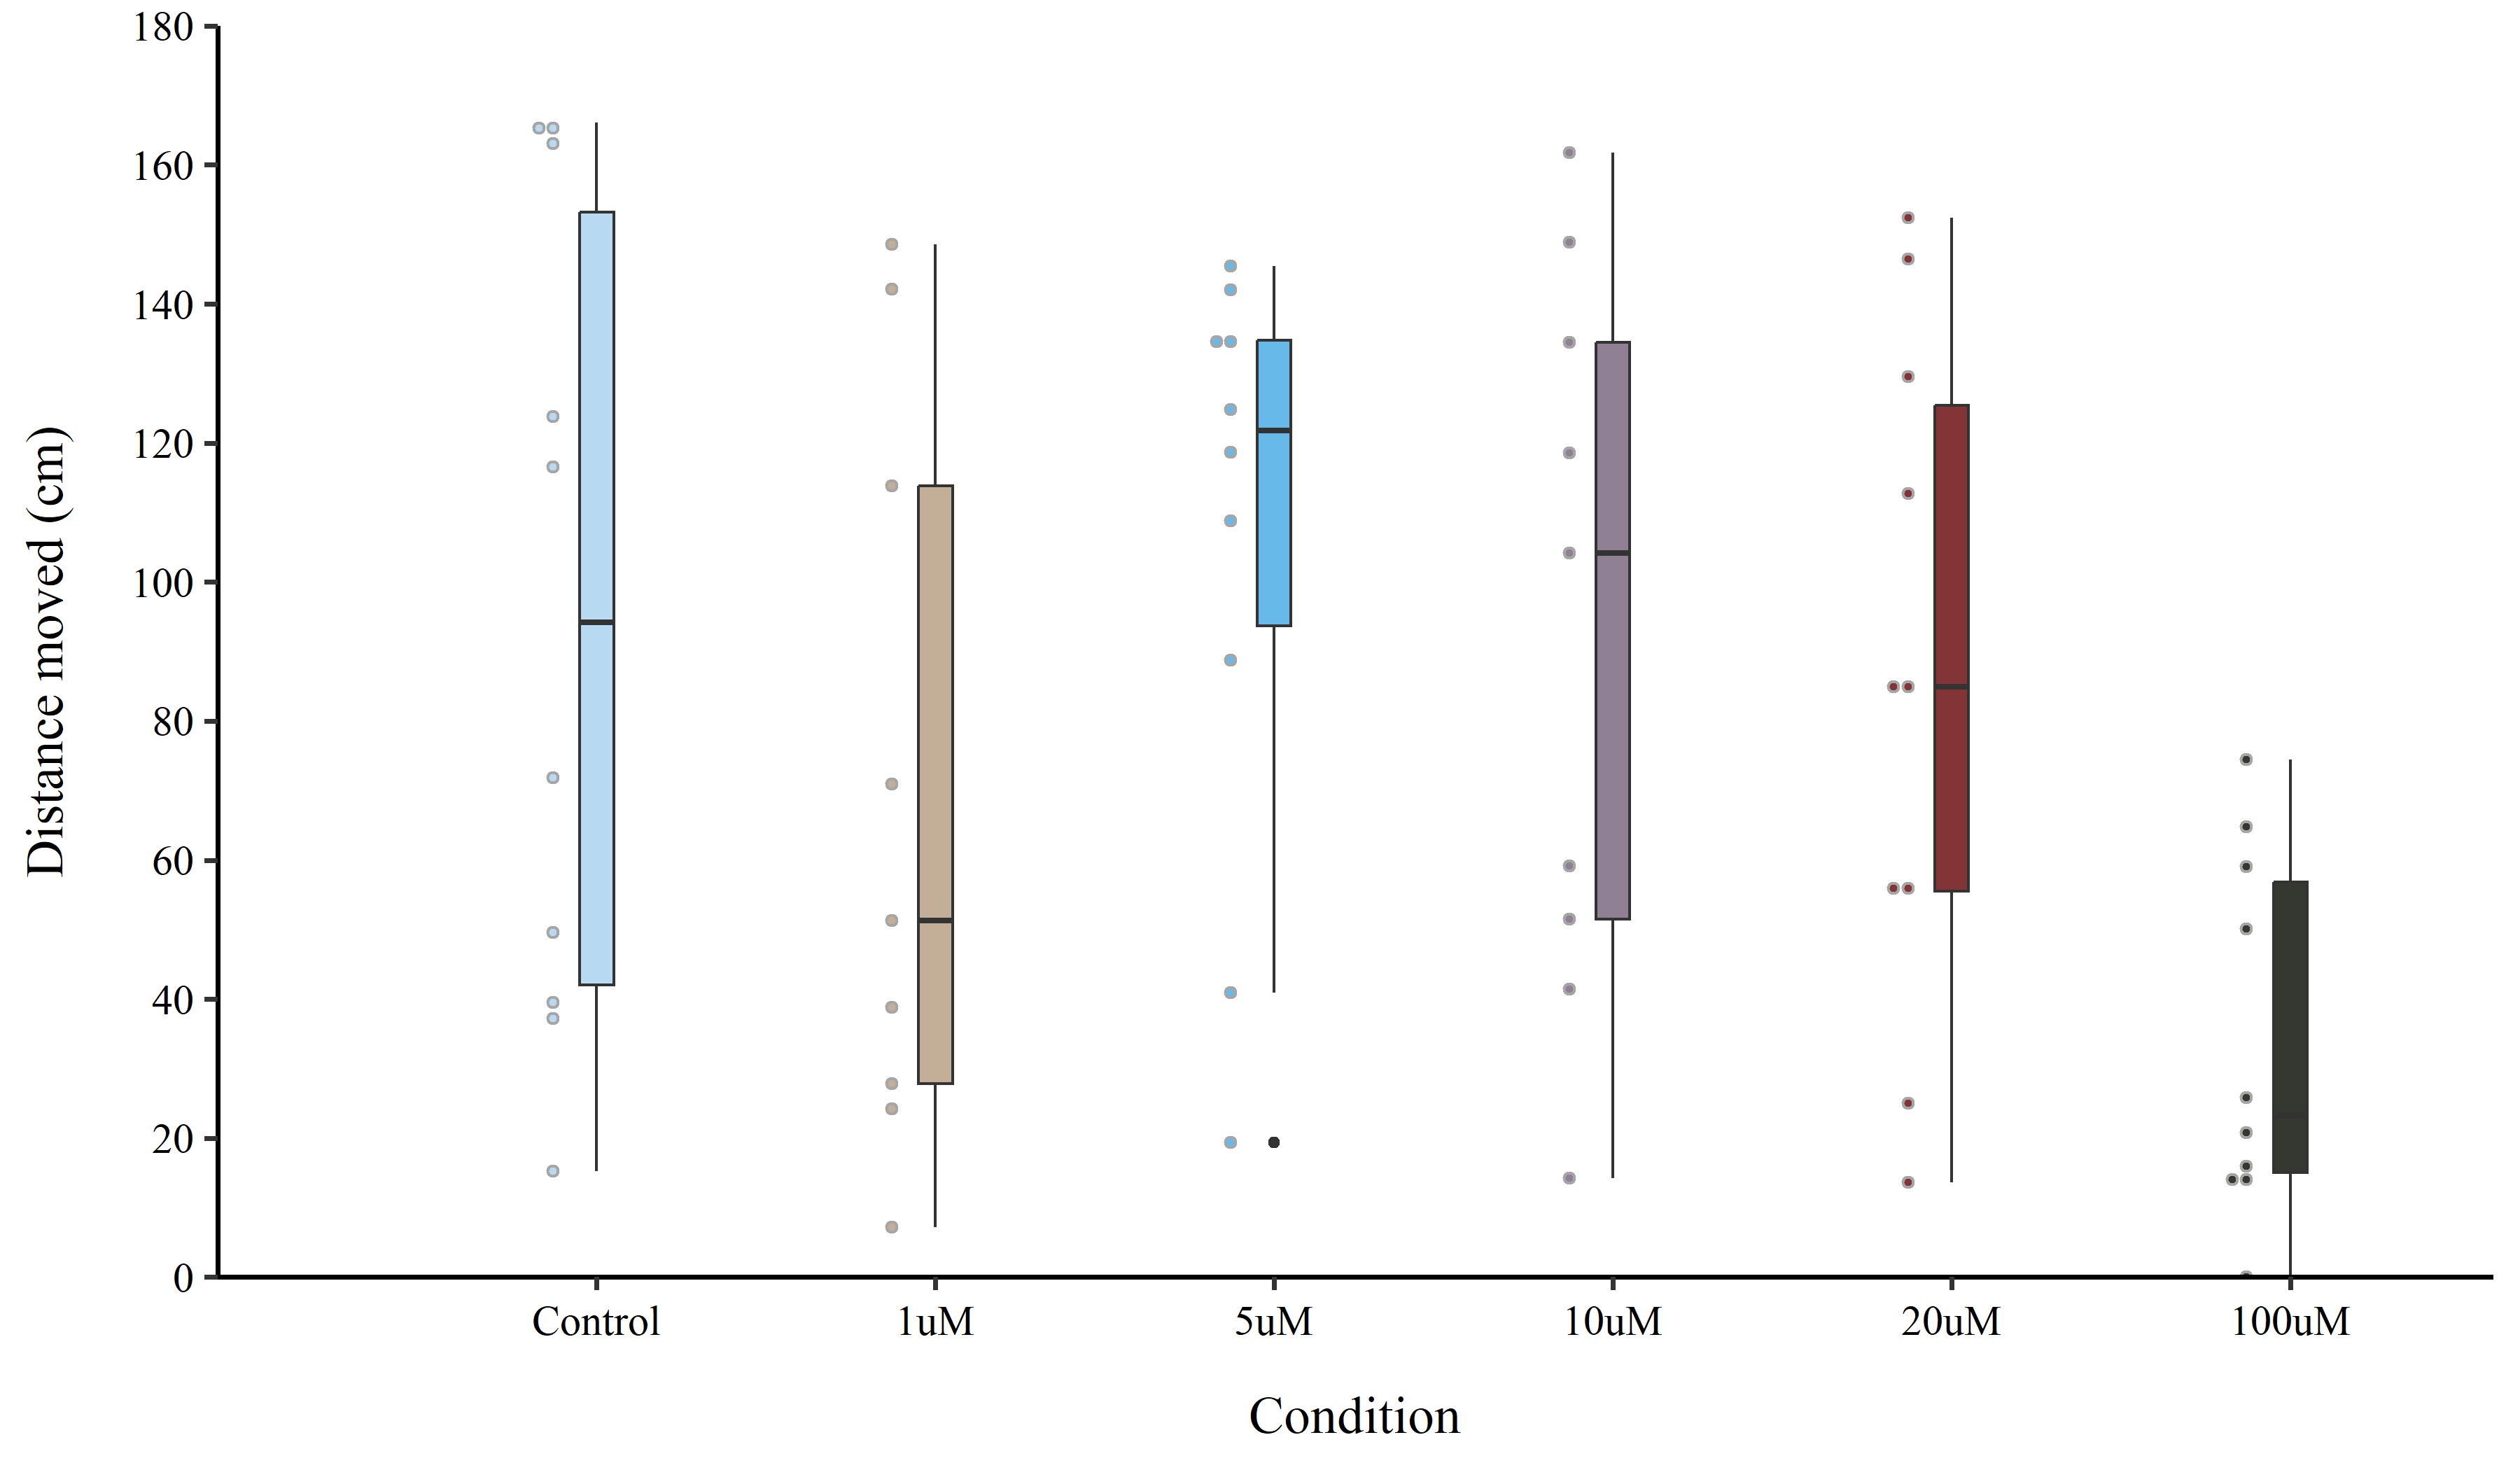
\includegraphics{Francis_Masters_Thesis_files/figure-pdf/fig-boxplot-1.png}

}

\caption{\label{fig-boxplot}Plot of planarian motility by condition}

\end{figure}%

The results in Figure~\ref{fig-boxplot} convey the variability of
planarian behaviour. All conditions had at least one subject which moved
less than 30cm over the 15 minute recording, and all groups had at least
two subjects that moved more than 140cm. Experimenter observations
indicate that when placed in the recording dish, some planaria --
typically those visible at the bottom of Figure~\ref{fig-boxplot} --
would move initially, and then come to rest within a few minutes at a
spot on the wall. They would remain here without meaningful movement for
the remainder of the recording. Although no statistically significant
difference was detected, there is a curious grouping of planaria in the
1μM condition below 60cm. Consistant with this, Hutchinson et al.~(2015)
observed a significant decrease in motility during exposure to 1μM of
cocaine but not to 10μM when compared to a control group. No potential
explanation was offered for this unusual dose-response effect. The most
likely explanation may be a type 1 error.

The dose-response results suggest that any of the proposed doses would
be appropriate for conditioning, in that they should not significantly
alter planarian behaviour. Because planaria will be exposed to multiple
trials within a short time interval, any effects on behaviour may mask
evidence of learning. But given this null dose-response result, the
primary selection criteria will now shift toward a focus on how
rewarding (and therefore reinforcing) the dose is. A range of cocaine
doses have been used to successfully condition planaria in CPP
paradigms. These procedures typically involve low doses such as 1μM
(Hutchinson et al., 2015), 5μM (Amaning-Kwarteng et al., 2017) or 10μM
(Hutchinson et al., 2015). But in the case of CPP, exposure time per
trial is relatively long, on the order of 15-20 minutes. In the operant
conditioning paradigm proposed in Experiment 2, exposure time will be 3
minutes. Similar levels of absorbtion given the time constraint may be
achieved by a higher concentration of the compound.

\begin{itemize}
\tightlist
\item
  Discuss 10\% average of missing frames.
\end{itemize}

\begin{figure}

\centering{

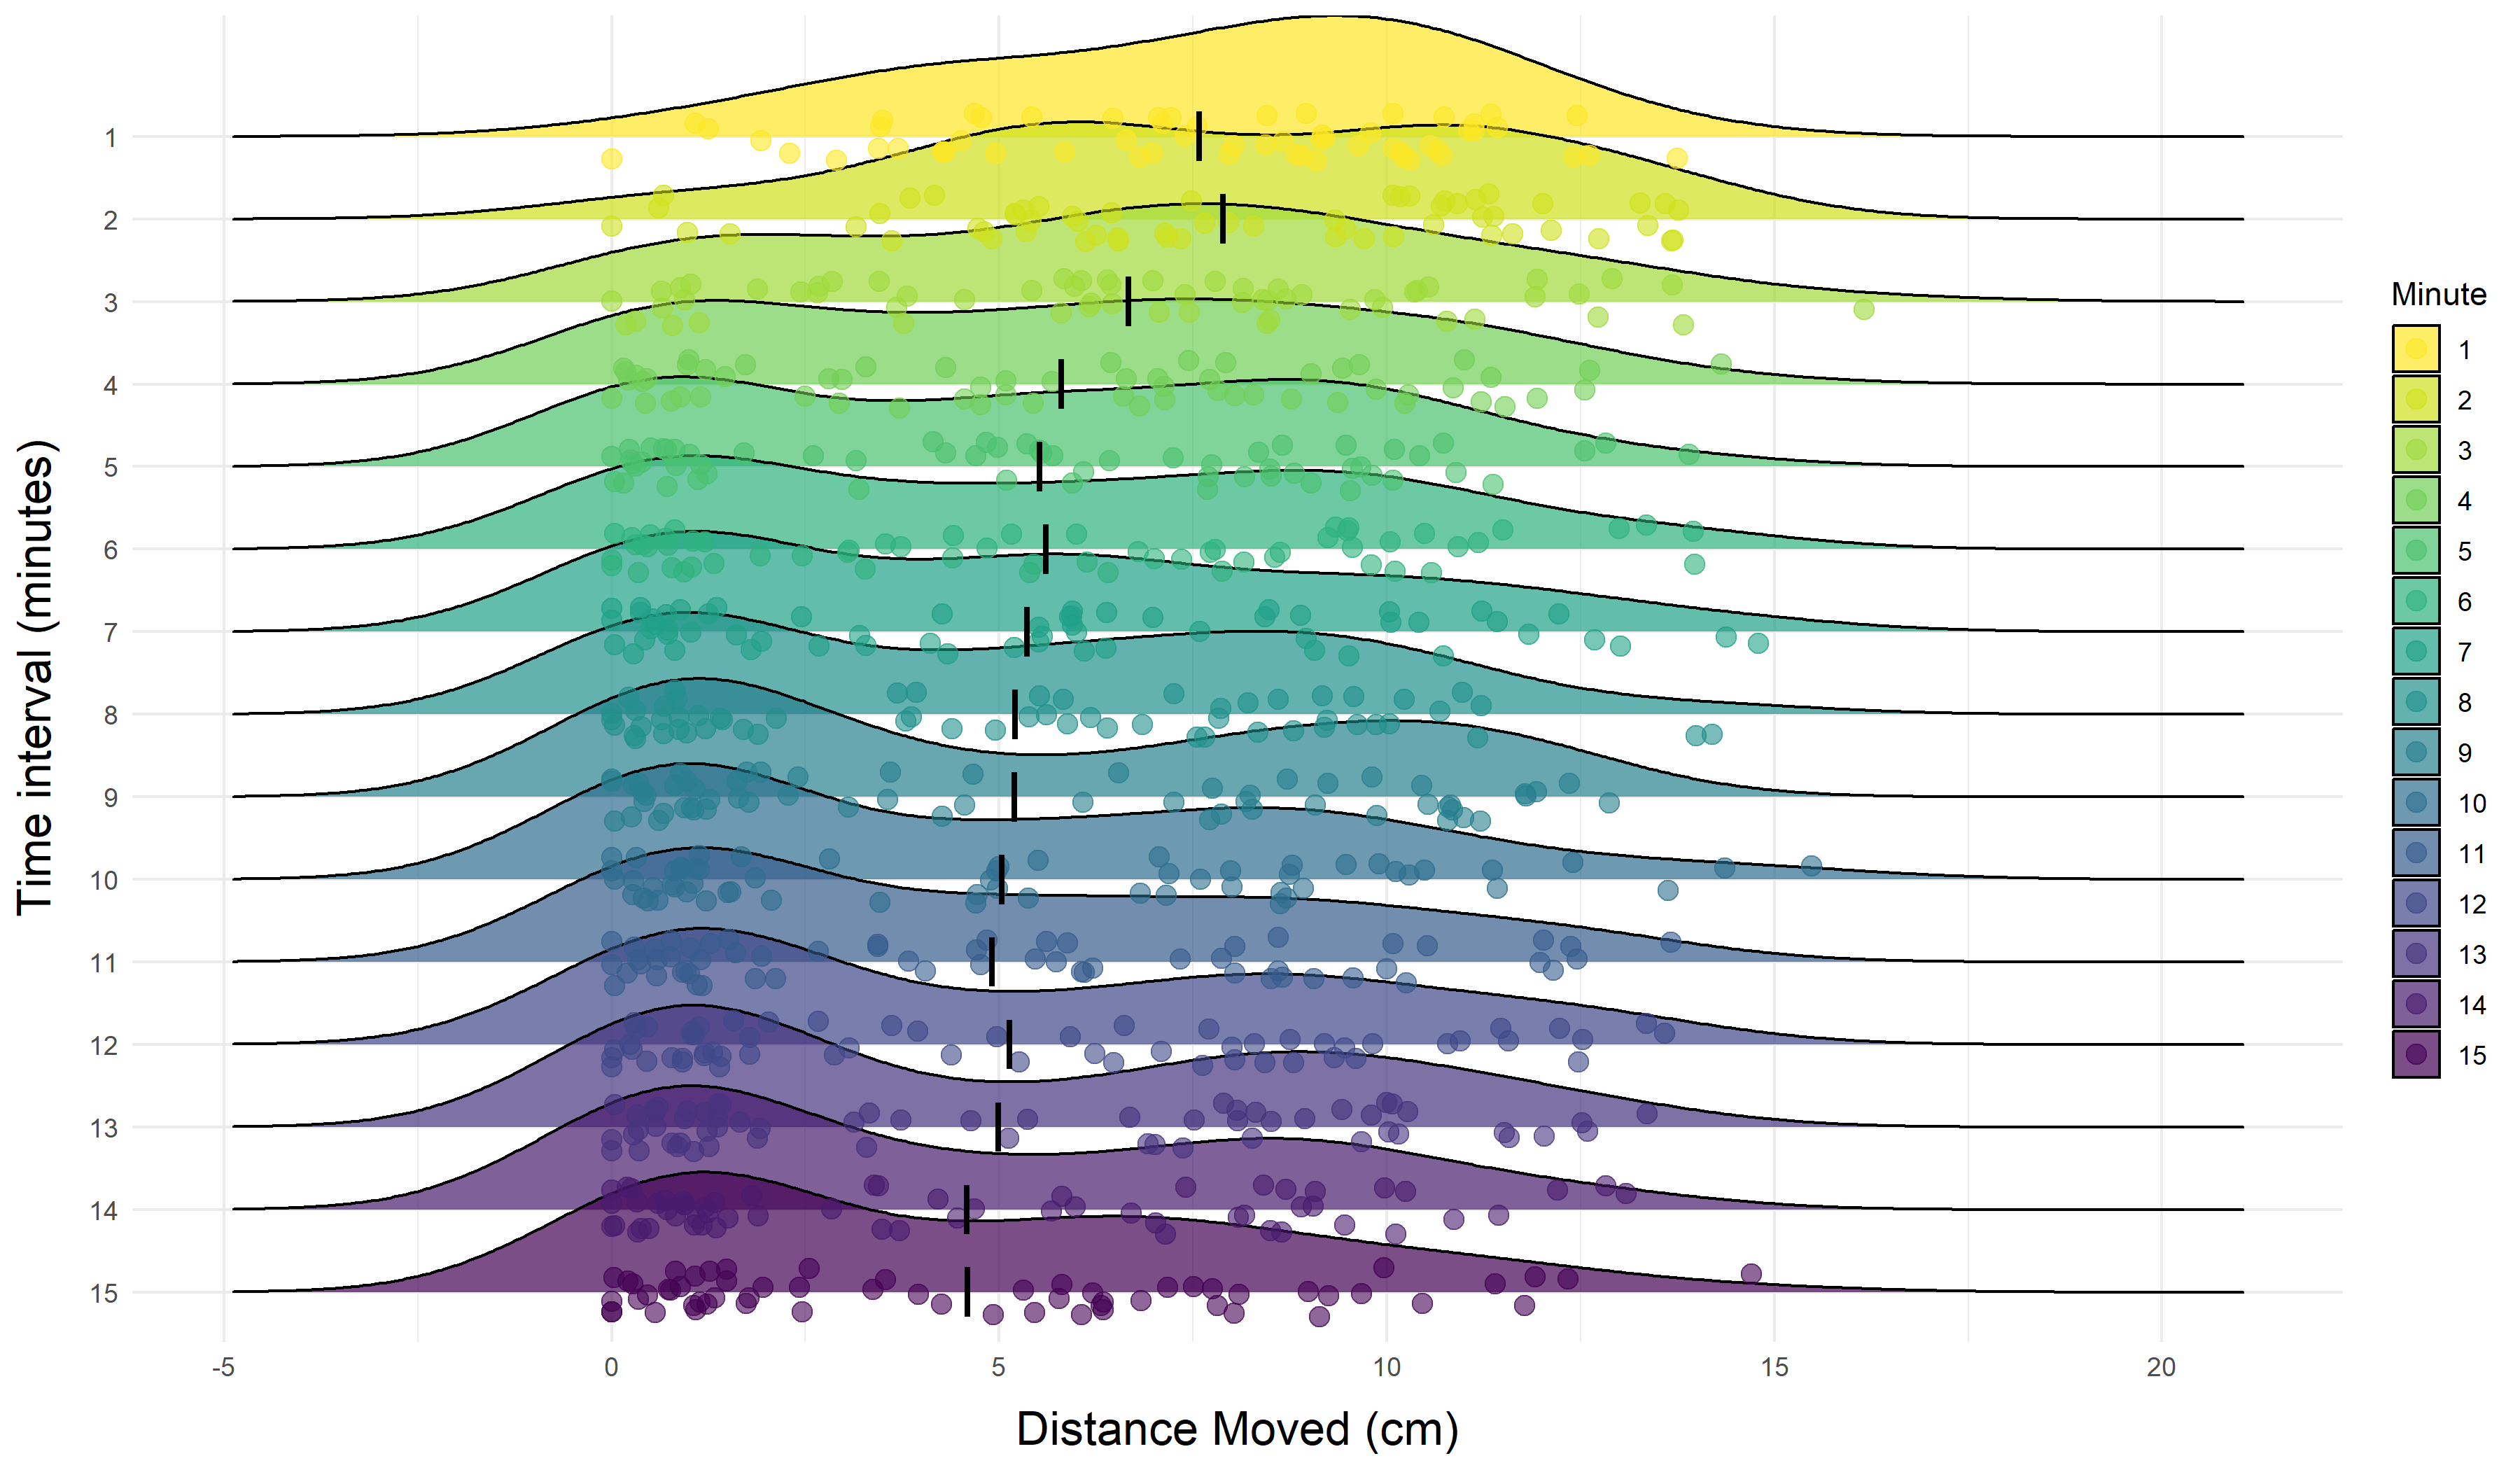
\includegraphics{Francis_Masters_Thesis_files/figure-pdf/fig-ridgeplot-1.png}

}

\caption{\label{fig-ridgeplot}Plot of planarian motility across
recording interval}

\end{figure}%

X

\subsection{Experiment 2}\label{experiment-2}

Next we sought to determine whether planaria can learn and retain an
operant conditioned response. Prior research has demonstrated the
capacity for learning by way of classical conditioning. And there is
evidence that classically conditioned memories can be retained after
decapitation and regeneration of the brain. But the capacity for complex
memories shaped by operant conditioning to persist despite losing most
of the central nervous system has not been definitively shown. As a
first step towards testing retention of operant conditioned memory, we
needed to first establish the capacity for operant learning in this
species of planaria. This experiment was preregistered prior to data
collection and can be found online at Open Science Framework
(\url{https://osf.io/tq7u4/?view_only=9c794dd942fb4a54b6a986c0a893fe46})
and at PsychArchives
(\url{https://www.psycharchives.org/en/item/d6109ed1-9aab-467b-b981-e009be95f308}

Sixty planaria were used (cocaine group, \emph{n} = 30, vehicle group,
\emph{n} = 30). This experiment had four stages: baseline, conditioning,
test, and priming. for baseline and conditioning two planaria were run
concurrently in two separate Y-mazes. The maze was filled with 1.8ml of
planaria water. The water was shaken so as to distribute evenly
throughout the maze, with bubbles removed as needed. Six planaria were
used per run, wherein they completed either 6 trials (baseline) or 4
trials per day (conditioning) with an intertrial interval of
approximately 15 minutes. The six planaria were first moved into holding
petri dishes, with the regular white room light on to encourage
movement. At the start of a trial, two planaria were transferred to the
middle of the runway using a paintbrush, and shaken loose into the
water. Once the planaria had entered the runway, the timer was started.
Planaria were given three minutes to enter one of the arms \^{}{[}If the
planarian had some part of their body in an arm, they would be given up
to an extra minute to make their decision{]}. Once a planarian had
enterd an arm, the plug was inserted to stop liquid moving between
compartments. Each arm contained 0.5ml after the plug was inserted. A
planarian was considered to have entered the arm when the plug could be
safely inserted without touching the planarian.

After plug insertion the timer was stopped, and the decision and time
were recorded on a computer. For treatment subjects, if the active arm
was selected, 43.5μL of cocaine in distilled water was pipetted near the
body. If the inactive arm was selected, an identical volume of distilled
water was pipetted near the body. After administration, the timer was
restarted and three minutes were given for absorption. For control
subjects, either arm resulted in plugging and then pipetting 43.5μL of
distilled water into the arm. If a subject failed to enter an arm, the
plug was inserted and 43.5μL of distilled water was pipetted near the
subjects body while in the runway and then three minutes were given. The
runway light was on throughout the duration of the trial. At the end of
a trial, planaria were gently removed and placed back into their holding
dish.

At test, six planaria were used per run. Three planaria were run
concurrently in three separate Y-mazes. Planaria were given three
minutes to make a decision. Once a decision was made, the plug was
inserted and planaria were left for \textasciitilde60 seconds before
being moved back to the holding dish. No additional liquid was added to
any compartment of the Y-maze during the test trials. The next group of
three planaria would then begin their first test trial. The inter trial
interval was approximately six minutes and thirty seconds. For the
priming stage, the procedure was identical to the test stage, with the
added component of the drug exposure before the first trial. At the
start of a run, the planaria were placed in a 8ml solution of cocaine
diluted in planaria water for 10 minutes (staggered so that subejcts 1-3
had finished their first trial before the 10-minute period ended for
subjects 4-6). At the end of the exposure interval, planaria were moved
individually into a Y-maze to begin their first trial. Planaria were
only exposed to cocaine before the first priming trial, but not before
subsequent trials.

\paragraph{Results and disciussion}\label{results-and-disciussion}

Figure~\ref{fig-Exp2-decisions-line} shows the average percentage of
trials where subjects entered the active arm across the four time
points. A generalised linear mixed effects model with family set to
binomial was fitted in R. Subject ID was set as a random effect, with
condition, time point and the interaction term as a fixed effects.
Pairwise comparisons with a Bonferroni correction were carried out using
the emmeans package in R. Type III Wald chi-square tests were carried
out to identify whether there was a main effect of condition, time, and
their interaction. The results did not find a significant effect of
condition (χ2 (1) = 0.773, p 0.379). The results indicate a significant
effect of time (χ2 (3) = 35.5, p = \textless.001) and a significant
time*condition interaction (χ2 (3) = 10.2, p = 0.0171)

\begin{figure}

\centering{

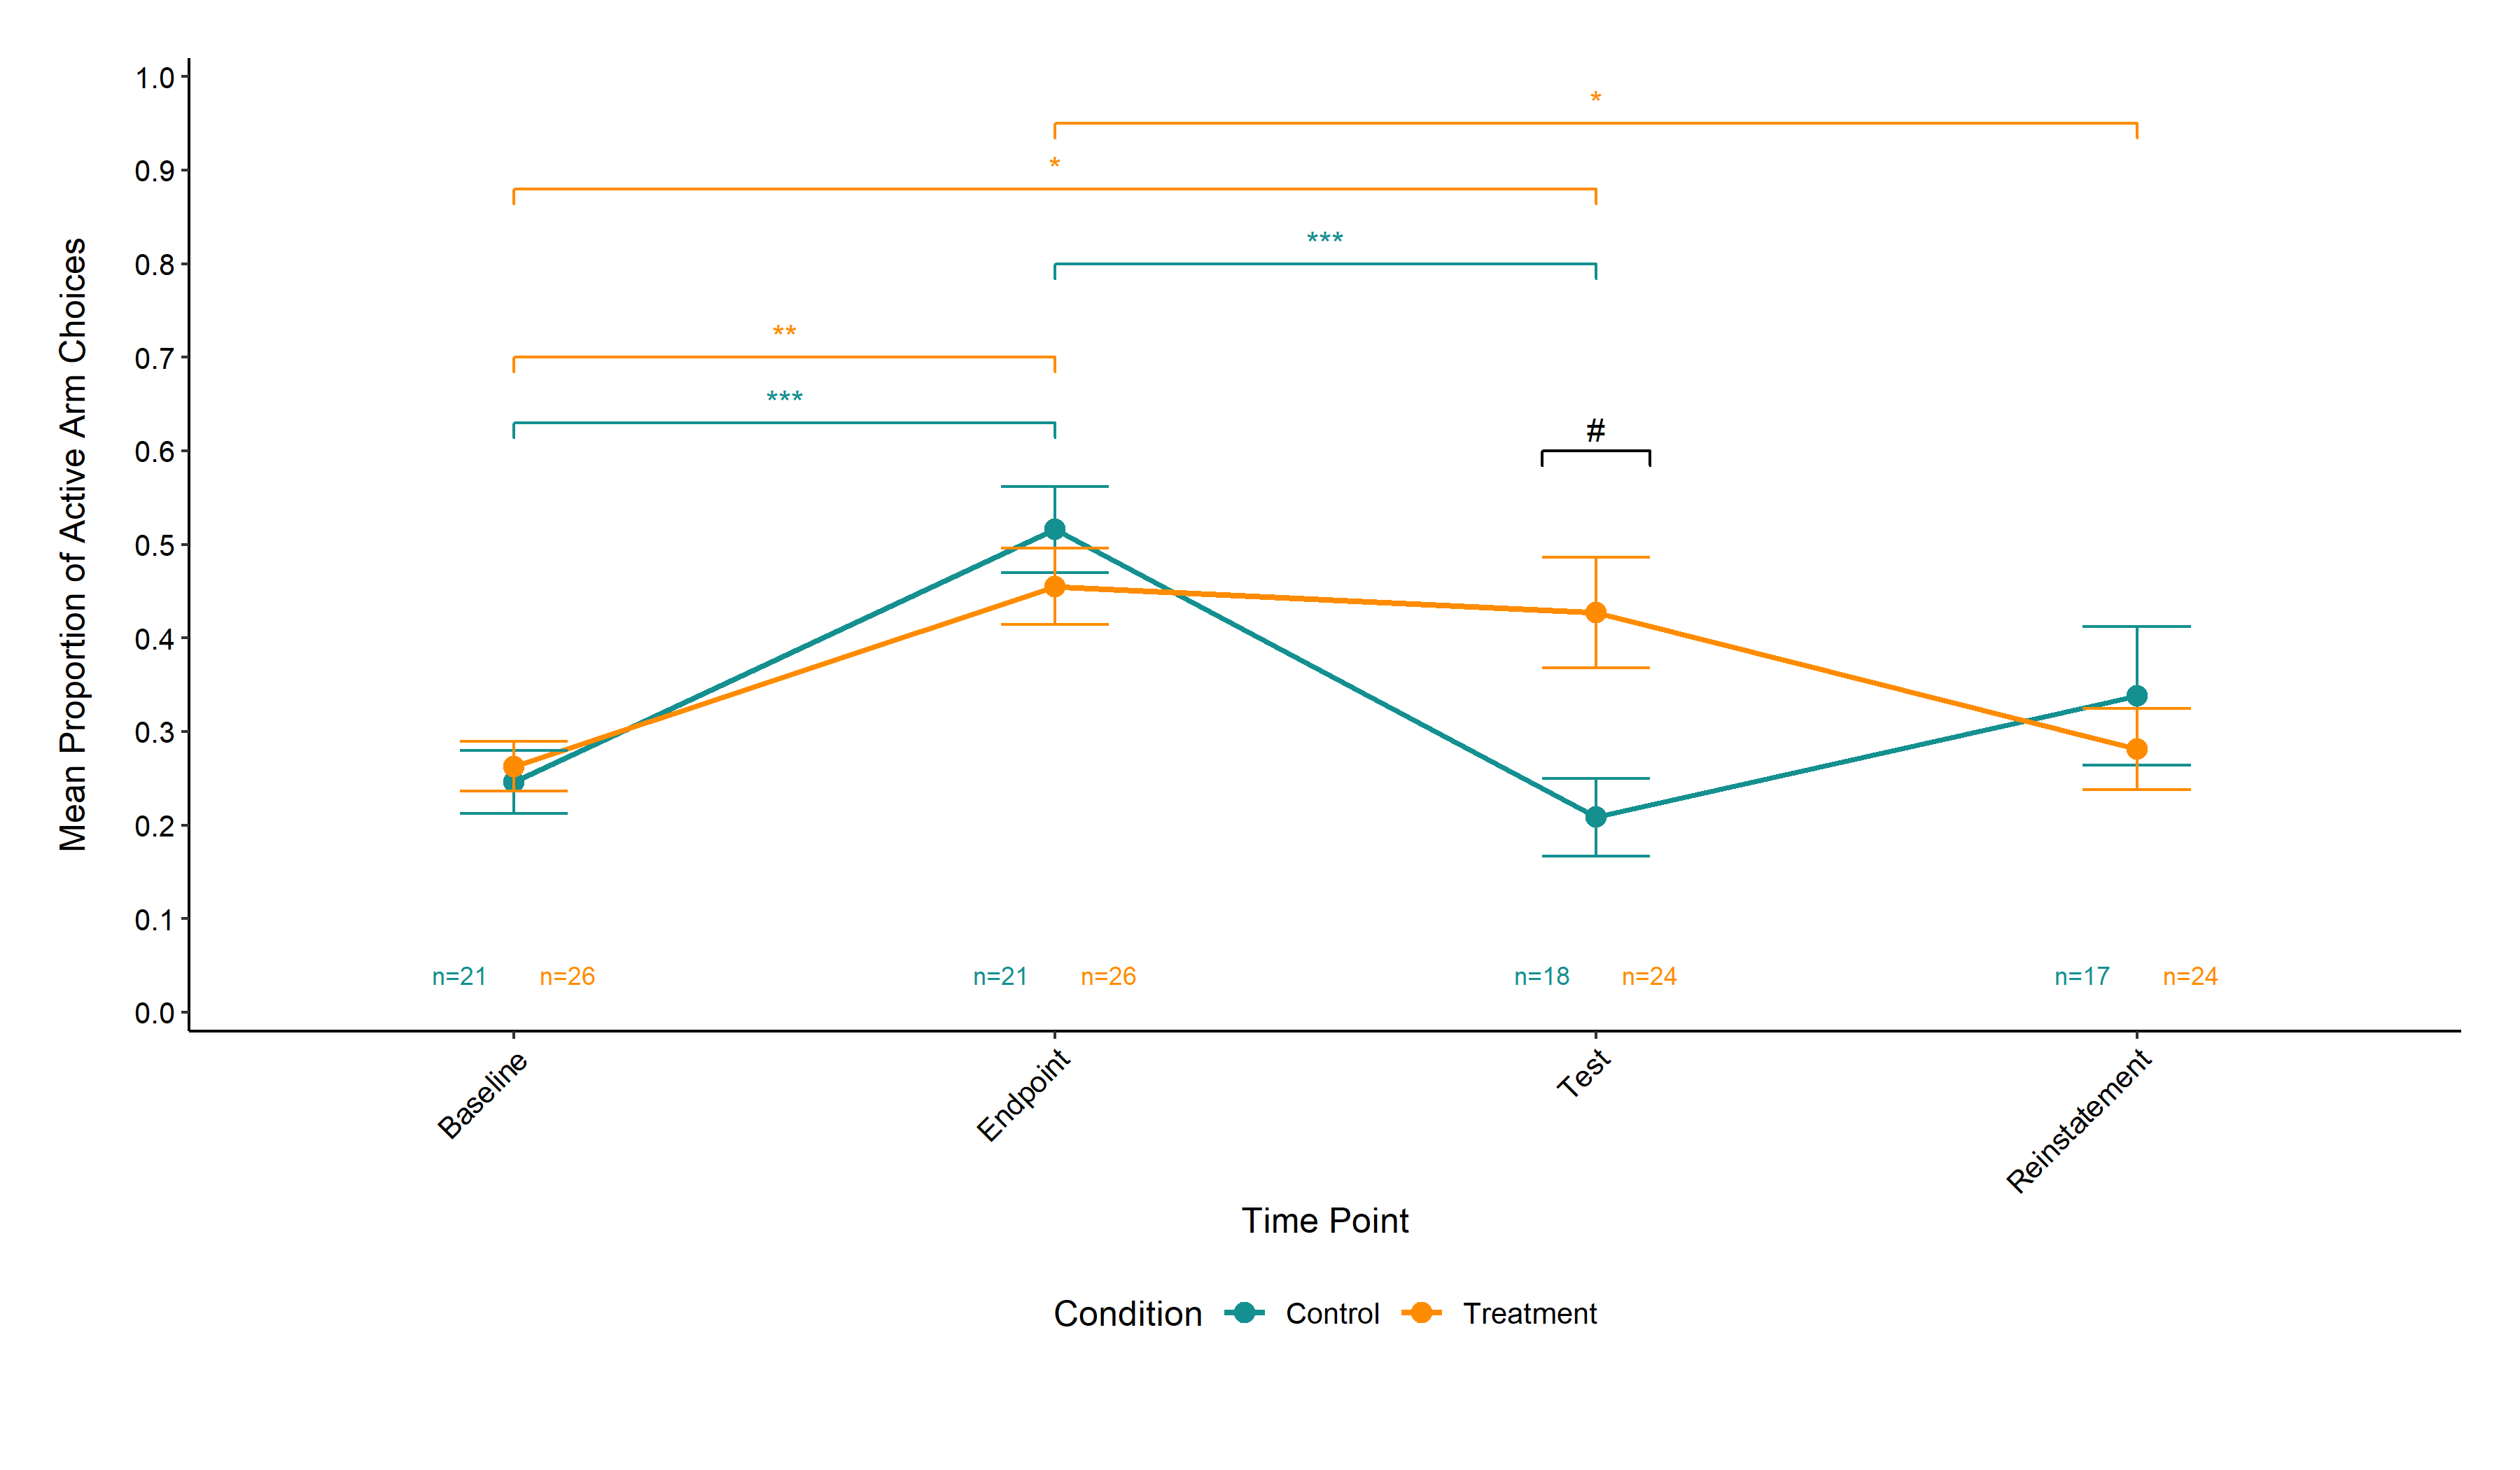
\includegraphics{Francis_Masters_Thesis_files/figure-pdf/fig-Exp2-decisions-line-1.png}

}

\caption{\label{fig-Exp2-decisions-line}Mean percentage of choices for
the active arm over time between conditions}

\end{figure}%

\newpage

This is my introductory paragraph. The title will be placed above it
automatically. \emph{Do not start with an introductory heading} (e.g.,
``Introduction''). The title acts as your Level 1 heading for the
introduction.

Details about writing headings with markdown in APA style are
\href{https://wjschne.github.io/apaquarto/writing.html\#headings-in-apa-style}{here}.

\subsection{Displaying Figures}\label{displaying-figures}

A reference label for a figure must have the prefix \texttt{fig-}, and
in a code chunk, the caption must be set with \texttt{fig-cap}. Captions
are in
\href{https://apastyle.apa.org/style-grammar-guidelines/capitalization/title-case}{title
case}.

To refer to any figure or table, use the \texttt{@} symbol followed by
the reference label (e.g., \textbf{?@fig-myplot}).

\subsection{Imported Graphics}\label{imported-graphics}

One way to import an existing graphic as a figure is to use
\texttt{knitr::include\_graphics} in a code chunk. For example,
\textbf{?@fig-import1} is an imported image. Note that in apaquarto-pdf
documents, we can specify that that a figure or table should span both
columns when in journal mode by setting the \texttt{apa-twocolumn} chunk
option to \texttt{true}. For other formats, this distinction does not
matter.

Figure graphics can be imported directly with Markdown, as with
Figure~\ref{fig-import2}.

\begin{figure}

\centering{

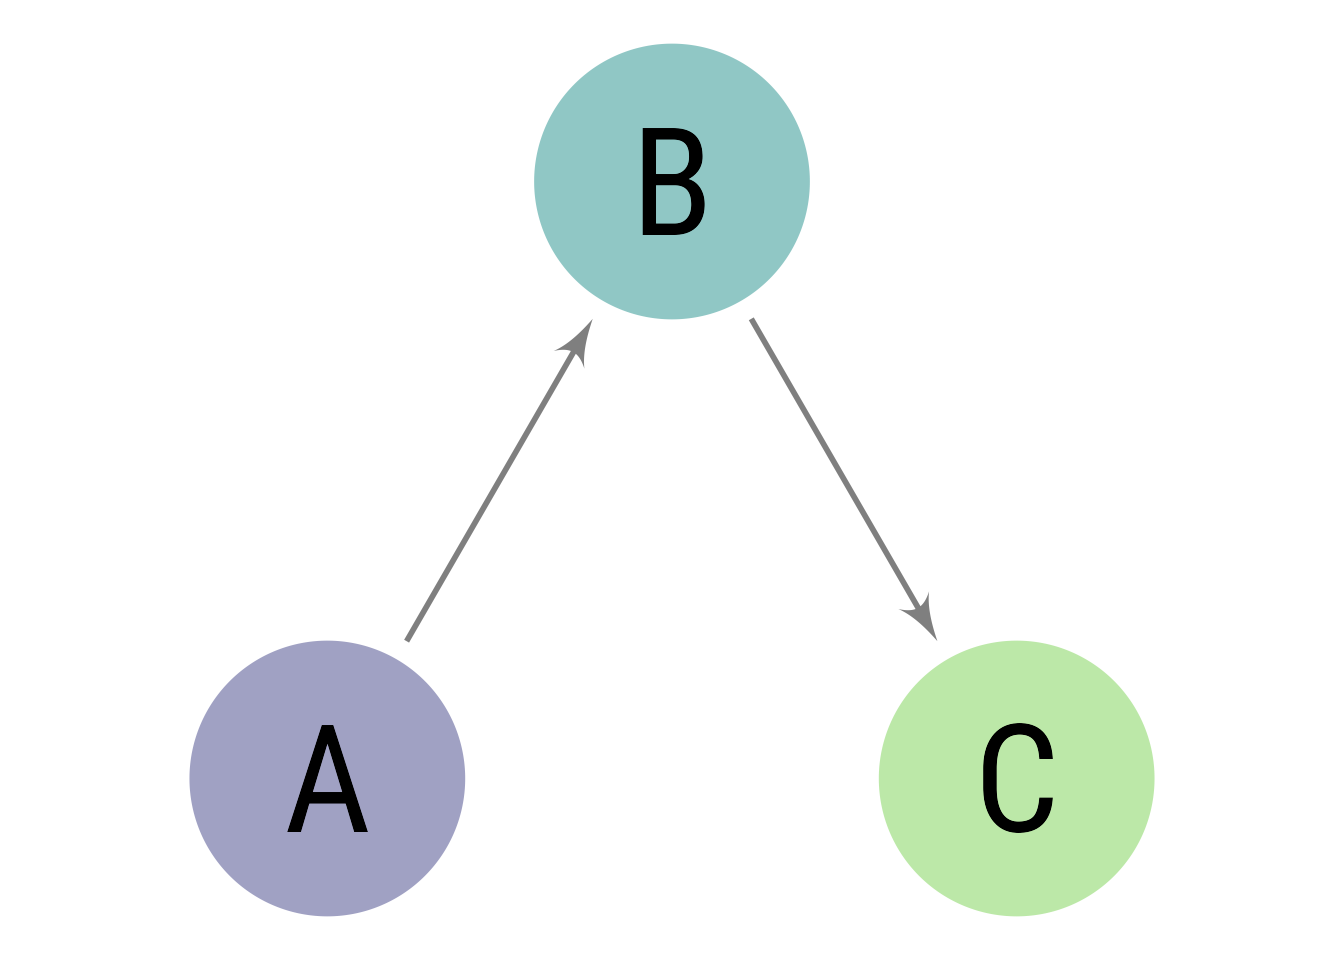
\includegraphics[width=0.49\textwidth,height=\textheight]{sampleimage.png}

}

\caption{\label{fig-import2}Another Way to Import Graphics}

\end{figure}%

Which style of creating figures you choose depends on preference and
need.

\subsection{Displaying Tables}\label{displaying-tables}

We can make a table the same way as a figure. Generating a table that
conforms to APA format in all document formats can be tricky. When the
table is simple, the \texttt{kable} function from knitr works well. Feel
free to experiment with different methods, but I have found that David
Gohel's \href{https://davidgohel.github.io/flextable/}{flextable} to be
the best option when I need something more complex.

To refer to this table in text, use the \texttt{@} symbol followed by
the reference label like so: As seen in Table~\ref{tbl-mytable}, the
first few numbers and letters of the alphabet are displayed.

In Table~\ref{tbl-mymarkdowntable}, there is an example of a plain
markdown table with a note below it.

\begin{longtable}[]{@{}llrc@{}}
\caption{Table Caption of a Markdown
Table}\label{tbl-mymarkdowntable}\tabularnewline
\toprule\noalign{}
Default & Left & Right & Center \\
\midrule\noalign{}
\endfirsthead
\toprule\noalign{}
Default & Left & Right & Center \\
\midrule\noalign{}
\endhead
\bottomrule\noalign{}
\endlastfoot
12 & 12 & 12 & 12 \\
123 & 123 & 123 & 123 \\
1 & 1 & 1 & 1 \\
\end{longtable}

What if you want the tables and figures to be at the end of the
document? In the .pdf format, you can set the \texttt{floatsintext}
option to false. For .html and .docx documents, there is not yet an
automatic way to put tables and figures at the end. You can, of course,
just put them all at the end, in order. The reference labels will work
no matter where they are in the text.

\subsection{Tables and Figures Spanning Two Columns in Journal
Mode}\label{tables-and-figures-spanning-two-columns-in-journal-mode}

When creating tables and figures in journal mode, care must be taken not
to make figures and tables wider than the columns, otherwise \(\LaTeX\)
sometimes makes them disappear.

As demonstrated in \textbf{?@fig-twocolumn}, you can make figures tables
span the two columns by setting the \texttt{apa-twocolumn} chunk option
to \texttt{true}.

\subsection{Math and Equations}\label{math-and-equations}

Inline math uses \(\LaTeX\) syntax with single dollar signs. For
example, the reliability coefficient of my measure is \(r_{XX}=.95\).

If you want to display and refer to a specific formula, enclose the
formula in two dollar signs. After the second pair of dollar signs,
place the label in curly braces. The label should have an \texttt{\#eq-}
prefix. To refer to the formula, use the same label but with the
\texttt{@} symbol. For example, Equation~\ref{eq-euler} is Euler's
Identity, which is much admired for its elegance.

\subsection{Citations}\label{citations}

See
\href{https://quarto.org/docs/authoring/footnotes-and-citations.html}{here}
for instructions on setting up citations and references.

A parenthetical citation requires square brackets
(\citeproc{ref-CameronTrivedi2013}{\textbf{CameronTrivedi2013?}}). This
reference was in my bibliography file. An in-text citation is done like
so:

(\citeproc{ref-CameronTrivedi2013}{\textbf{CameronTrivedi2013?}}) make
some important points \ldots{}

See
\href{https://wjschne.github.io/apaquarto/writing.html\#references}{here}
for explanations, examples, and citation features exclusive to
apaquarto. For example, apaquarto can automatically handle possessive
citations:

(\citeproc{ref-schneider2012cattell}{\textbf{schneider2012cattell?}}'s)
position was \ldots{}

\subsection{Masking Author Identity for Peer
Review}\label{masking-author-identity-for-peer-review}

Setting \texttt{mask} to \texttt{true} will remove author names,
affiliations, and correspondence from the title page. Any references
listed in the \texttt{masked-citations} field will be masked as well.
See
\href{https://wjschne.github.io/apaquarto/writing.html\#masked-citations-for-anonymous-peer-review}{here}
for more information.

\begin{equation}\phantomsection\label{eq-euler}{
e^{i\pi}+1=0
}\end{equation}

\subsection{Block Quotes}\label{block-quotes}

Sometimes you want to give a longer quote that needs to go in its own
paragraph. Block quotes are on their own line starting with the
\textgreater{} character. For example,
(\citeproc{ref-austenMansfieldPark1990}{\textbf{austenMansfieldPark1990?}}'s)
\emph{Mansfield Park} has some memorable insights about the mind:

\begin{quote}
If any one faculty of our nature may be called more wonderful than the
rest, I do think it is memory. There seems something more speakingly
incomprehensible in the powers, the failures, the inequalities of
memory, than in any other of our intelligences. The memory is sometimes
so retentive, so serviceable, so obedient; at others, so bewildered and
so weak; and at others again, so tyrannic, so beyond control! We are, to
be sure, a miracle every way; but our powers of recollecting and of
forgetting do seem peculiarly past finding out. (p.~163)
\end{quote}

If your quote has multiple paragraphs, like this passage from
(\citeproc{ref-brownHowKilledPluto2012}{\textbf{brownHowKilledPluto2012?}}),
separate them with a lone \texttt{\textgreater{}} character between the
lines:

\begin{quote}
In the entire field of astronomy, there is no word other than
\emph{planet} that has a precise, lawyerly definition, in which certain
criteria are specifically enumerated. Why does \emph{planet} have such a
definition but \emph{star}, \emph{galaxy}, and \emph{giant molecular
cloud} do not? Because in astronomy, as in most sciences, scientists
work by concepts rather than by definitions. The concept of a star is
clear; a star is a collection of gas with fusion reactions in the
interior giving off energy. A galaxy is a large, bound collection of
stars. A giant molecular cloud is a giant cloud of molecules. The
concept of a planet---in the eight-planet solar system---is equally
simple to state. A planet is a one of a small number of bodies that
dominate a planetary system. That is a concept, not a definition. How
would you write that down in a precise definition?

I wouldn't. Once you write down a definition with lawyerly precision,
you get the lawyers involved in deciding whether or not your objects are
planets. Astronomers work in concepts. We rarely call in the attorneys
for adjudication. (p.~242)
\end{quote}

\subsection{Hypotheses, Aims, and
Objectives}\label{hypotheses-aims-and-objectives}

The last paragraph of the introduction usually states the specific
hypotheses of the study, often in a way that links them to the research
design.

\section{Method}\label{method}

General remarks on method. This paragraph is optional.

Not all papers require each of these sections. Edit them as needed.
Consult the \href{https://apastyle.apa.org/jars}{Journal Article
Reporting Standards} for what is needed for your type of article.

\subsection{Participants}\label{participants}

Who are they? How were they recruited? Report criteria for participant
inclusion and exclusion. Perhaps some basic demographic stats are in
order. A table is a great way to avoid repetition in statistical
reporting.

\subsection{Measures}\label{measures}

This section can also be titled \textbf{Materials} or
\textbf{Apparatus}. Whatever tools, equipment, or measurement devices
used in the study should be described.

\subsubsection{Measure A}\label{measure-a}

Describe Measure A.

\subsubsection{Measure B}\label{measure-b}

Describe Measure B.

\paragraph{Subscale B1}\label{subscale-b1}

A paragraph after a 4th-level header will appear on the same line as the
header.

\paragraph{Subscale B2}\label{subscale-b2}

A paragraph after a 4th-level header will appear on the same line as the
header.

\subparagraph{Subscale B2a}\label{subscale-b2a}

A paragraph after a 5th-level header will appear on the same line as the
header.

\subparagraph{Subscale B2b}\label{subscale-b2b}

A paragraph after a 5th-level header will appear on the same line as the
header.

\subsection{Procedure}\label{procedure}

What did participants do? How are the data going to be analyzed?

\section{Results}\label{results-1}

\subsection{Descriptive Statistics}\label{descriptive-statistics}

Describe the basic characteristics of the primary variables. My ideal is
to describe the variables well enough that someone conducting a
meta-analysis can include the study without needing to ask for
additional information.

\section{Discussion}\label{discussion}

Describe results in non-statistical terms.

\subsection{Limitations and Future
Directions}\label{limitations-and-future-directions}

Every study has limitations. Based on this study, some additional steps
might include\ldots{}

\subsection{Conclusion}\label{conclusion}

Describe the main point of the paper.

\section{References}\label{references}

\phantomsection\label{refs}
\begin{CSLReferences}{1}{0}
\bibitem[\citeproctext]{ref-algeri1983}
Algeri, Sergio, Antonio Carolei, Patrizia Ferretti, Claudia Gallone,
Guido Palladini, and Giorgio Venturini. 1983. {``Effects of Dopaminergic
Agents on Monoamine Levels and Motor Behaviour in Planaria.''}
\emph{Comparative Biochemistry and Physiology Part C: Comparative
Pharmacology} 74 (1): 27--29.
\url{https://doi.org/10.1016/0742-8413(83)90142-1}.

\bibitem[\citeproctext]{ref-barron_embracing_2015}
Barron, Andrew B, Eileen A Hebets, Thomas A Cleland, Courtney L
Fitzpatrick, Mark E Hauber, and Jeffrey R Stevens. 2015. {``Embracing
Multiple Definitions of Learning.''} \emph{Trends in Neurosciences
(Regular Ed.)} 38 (7): 405--7.
\url{https://doi.org/10.1016/j.tins.2015.04.008}.

\bibitem[\citeproctext]{ref-buttarelli_neuropharmacology_2008}
Buttarelli, Francesca R., Clelia Pellicano, and Francesco E. Pontieri.
2008. {``Neuropharmacology and Behavior in Planarians: {Translations} to
Mammals.''} \emph{Comparative Biochemistry and Physiology Part C:
Toxicology \& Pharmacology} 147 (4): 399--408.
\url{https://doi.org/10.1016/j.cbpc.2008.01.009}.

\bibitem[\citeproctext]{ref-cochet-escartin2015}
Cochet-Escartin, Olivier, Keith J Mickolajczyk, and Eva-Maria S Collins.
2015. {``Scrunching: A Novel Escape Gait in Planarians.''}
\emph{Physical Biology} 12 (5): 056010.
\url{https://doi.org/10.1088/1478-3975/12/5/056010}.

\bibitem[\citeproctext]{ref-debold1965}
DeBold, R. C., W. R. Thompson, and C. Landraitis. 1965. {``Differences
in Responses to Light Between Two Species of Planaria: Dugesis Tigrina
and d. Dorotocephala.''} \emph{Psychonomic Science} 2 (1): 79--80.
\url{https://doi.org/10.3758/BF03343339}.

\bibitem[\citeproctext]{ref-ermakov_planarians_2021}
Ermakov, Artem M., Kristina A. Kamenskikh, Olga N. Ermakova, Artem S.
Blagodatsky, Anton L. Popov, and Vladimir K. Ivanov. 2021. {``Planarians
as an {In} {Vivo} {Experimental} {Model} for the {Study} of {New}
{Radioprotective} {Substances}.''} \emph{Antioxidants} 10 (11).
\url{https://doi.org/10.3390/antiox10111763}.

\bibitem[\citeproctext]{ref-hagstrom2019}
Hagstrom, Danielle, Lisa Truong, Siqi Zhang, Robert Tanguay, and
Eva-Maria S Collins. 2019. {``Comparative Analysis of Zebrafish and
Planarian Model Systems for Developmental Neurotoxicity Screens Using an
87-Compound Library.''} \emph{Toxicological Sciences} 167 (1): 15--25.
\url{https://doi.org/10.1093/toxsci/kfy180}.

\bibitem[\citeproctext]{ref-hoerl2019}
Hoerl, Christoph, and Teresa McCormack. 2019. {``Thinking in and about
Time: A Dual Systems Perspective on Temporal Cognition.''}
\emph{Behavioral and Brain Sciences} 42: e244.
\url{https://doi.org/10.1017/S0140525X18002157}.

\bibitem[\citeproctext]{ref-karami2015}
Karami, Ali, Hamid Tebyanian, Vahabodin Goodarzi, and Sajad Shiri. 2015.
{``Planarians: An in Vivo Model for Regenerative Medicine.''}
\emph{International Journal of Stem Cells} 8: 128--33.
\url{https://api.semanticscholar.org/CorpusID:15186660}.

\bibitem[\citeproctext]{ref-li2008}
Li, Mei-Hui. 2008. {``Effects of Nonionic and Ionic Surfactants on
Survival, Oxidative Stress, and Cholinesterase Activity of Planarian.''}
\emph{Chemosphere} 70 (10): 1796--1803.
\url{https://doi.org/10.1016/j.chemosphere.2007.08.032}.

\bibitem[\citeproctext]{ref-miller_timescales_2024}
Miller, Jacob A., and Christos Constantinidis. 2024. {``Timescales of
Learning in Prefrontal Cortex.''} \emph{Nature Reviews Neuroscience},
June. \url{https://doi.org/10.1038/s41583-024-00836-8}.

\bibitem[\citeproctext]{ref-raffa2008}
Raffa, Robert B. 2008. \emph{Planaria: A Model for Drug Action and
Abuse}. First edition. Molecular Biology Intelligence Unit. Boca Raton,
FL: CRC Press, an imprint of Taylor; Francis.

\bibitem[\citeproctext]{ref-schacter_memory_1994}
Schacter, Daniel L., and Endel Tulving. 1994. \emph{Memory Systems
1994}. Cambridge, Mass: MIT Press.

\bibitem[\citeproctext]{ref-squire_memory_1987}
Squire, Larry R. 1987. \emph{Memory and Brain.} Memory and Brain. New
York, NY, US: Oxford University Press.

\bibitem[\citeproctext]{ref-tulving2005}
Tulving, Endel. 2005. {``3Episodic Memory and Autonoesis: Uniquely
Human?''} In, edited by Herbert S. Terrace and Janet Metcalfe, 0. Oxford
University Press.
\url{https://doi.org/10.1093/acprof:oso/9780195161564.003.0001}.

\bibitem[\citeproctext]{ref-vistassepmission11team2018}
Vista SSEP Mission 11 Team, Danielle Hagstrom, Christine Bartee, and
Eva-Maria S. Collins. 2018. {``Studying Planarian Regeneration Aboard
the International Space Station Within the Student Space Flight
Experimental Program.''} \emph{Frontiers in Astronomy and Space
Sciences} 5 (May): 12. \url{https://doi.org/10.3389/fspas.2018.00012}.

\end{CSLReferences}

\section{Appendix}\label{appendix}

\section{The Title for Appendix}\label{the-title-for-appendix}

If there are multiple appendices, label them with level 1 headings as
Appendix A, Appendix B, and so forth.

Tables and figures in the first appendix automatically get the prefix
``A'', and the numbering starts again at 1. See
Figure~\ref{fig-appendfig}.

If there were a second appendix, tables and figures would get the prefix
``B'', and the numbering starts again at 1. Make as many appendices as
needed.

\begin{figure}

\centering{

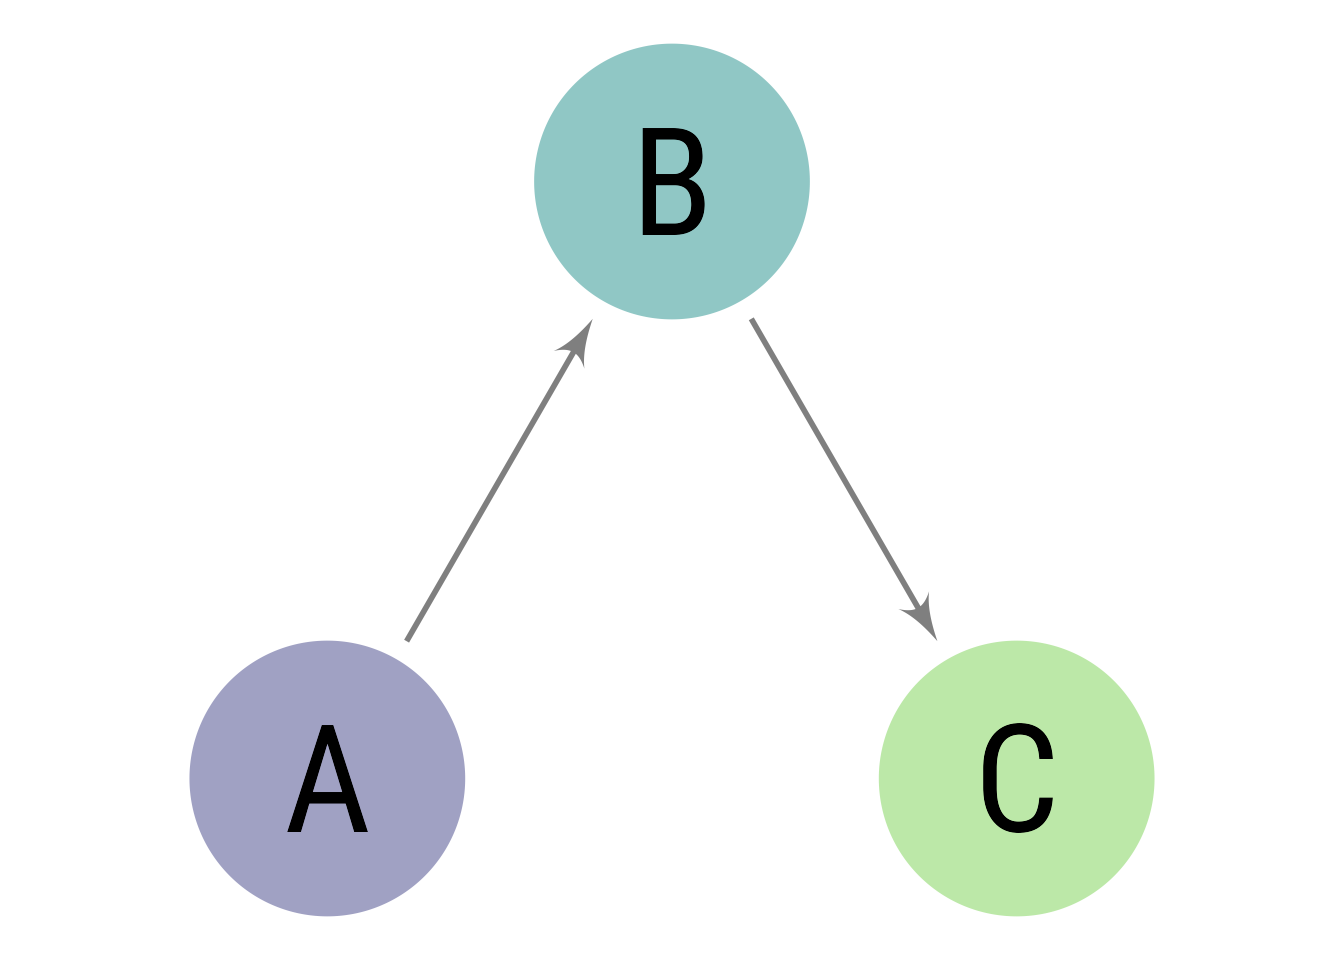
\includegraphics{sampleimage.png}

}

\caption{\label{fig-appendfig}Appendix Figure}

\end{figure}%

\subsection{Graveyard}\label{graveyard}

.Some common examples of invertebrates studied within psychology include
flies, bees, worms, and octopi

Planarians are thought to have existed for approximately 300 million
years (Vila-Farré \& Rink, 2018).

This allowed fine-grained control of experimental variables to minimise
variability across trials.




\end{document}
